\documentclass[11pt]{article}
\usepackage[a4paper,margin=24mm]{geometry}
\usepackage{amsmath,amssymb,amsthm,booktabs,longtable,array,graphicx,hyperref}
\usepackage[T1]{fontenc}
\usepackage{lmodern}
\hypersetup{colorlinks=true,linkcolor=black,urlcolor=blue}
\setlength{\emergencystretch}{2em}
\renewcommand{\topfraction}{0.9}\renewcommand{\bottomfraction}{0.8}\renewcommand{\textfraction}{0.1}\renewcommand{\floatpagefraction}{0.85}
\renewcommand{\thesection}{\Alph{section}}
\renewcommand{\thetable}{S\arabic{table}}
\renewcommand{\thefigure}{S\arabic{figure}}
\renewcommand{\theequation}{\thesection.\arabic{equation}}
\renewcommand{\theHequation}{\thesection.\arabic{equation}}
\newenvironment{widefigure}[1][]{\begin{figure}[#1]}{\end{figure}}
\newenvironment{widetable}[1][]{\begin{table}[#1]}{\end{table}}
\newcommand{\E}{\mathbb E}
\newcommand{\PP}{\mathbb P}
\title{Online Supplement\\[6pt]\large Low-Dimensional Asset-Pricing Networks: Identification, Stability, and Economic Use}
\author{}
\date{}
\begin{document}
\maketitle
\vspace{-2em}
This supplement records the estimator definitions, proof, chronology qualifications, and expanded numerical tables behind the article. Electronic long tables retain every archived condition; accompanying CSV files also retain the empirical seed-level distances. The original experiments are retained. A later bounded supplement adds a matched random-network control and a same-panel six-feature ablation; their protocols and chronology are stated separately. Protocol identifiers below are archival keys, not names of externally registered studies.

\section{Known-loading selection result}
\setcounter{equation}{0}
Let the finite ordered candidate set $\mathcal K$ contain $K_0$ and at least one larger dimension. Let $B$ be a fixed full-column-rank matrix and $B_K$ its first $K$ columns. For fixed $W\succ0$, define
\begin{equation}
P_K=B_K(B_K'WB_K)^{-1}B_K'W.
\end{equation}
Then $P_K^2=P_K$, $P_K'W=WP_K$, and, for $K>K_0$, $Q_K=P_K-P_{K_0}$ is also a $W$-orthogonal projector, with $Q_KP_{K_0}=P_{K_0}Q_K=0$. Suppose the fixed population mean $\mu$ belongs to the span of $B_{K_0}$ but to none of the smaller candidate spans. Training and evaluation sample means are independent:
\begin{equation}
\bar R_n=\mu+U/\sqrt n,\qquad \bar R_T^e=\mu+V/\sqrt T,
\qquad U,V\stackrel{ind}{\sim}N(0,\Sigma),\quad\Sigma\succ0.
\end{equation}
The training estimate is $\widehat\mu_K=P_K\bar R_n$, and validation loss is $L_T(K)=\|\bar R_T^e-\widehat\mu_K\|_W^2$. Ties are resolved in favor of the smaller dimension. The asymptotic sequence holds $B,W,\Sigma,\mu$ and $\mathcal K$ fixed, with $n/T\to c\in(0,\infty)$.

\subsection{Exact loss difference and nonvanishing over-selection}
For $K\ge K_0$, $P_K\mu=\mu$, so
\begin{equation}
L_T(K)=\|V/\sqrt T-P_KU/\sqrt n\|_W^2.
\end{equation}
Using $P_K=P_{K_0}+Q_K$ and orthogonality, expansion gives
\begin{equation}
T\{L_T(K)-L_T(K_0)\}=(T/n)U'Q_K'WQ_KU-2\sqrt{T/n}\,V'WQ_KU.
\label{eq:s-exact}
\end{equation}
It converges in distribution to
\begin{equation}
Z_K=c^{-1}\|Q_KU\|_W^2-2c^{-1/2}V'WQ_KU.
\end{equation}
Because $Q_K$ has positive rank and $U$ has a nonsingular Gaussian distribution, $q=Q_KU\ne0$ almost surely. Conditional on $U$, $V'Wq$ is normal with zero mean and strictly positive variance $q'W\Sigma Wq$. Consequently
\begin{equation}
\PP(Z_K<0\mid U)=1-\Phi\!\left(\frac{\|q\|_W^2}{2\sqrt c\sqrt{q'W\Sigma Wq}}\right)>0
\end{equation}
almost surely. The mixture has no atom at zero. Thus $\PP(L_T(K)<L_T(K_0))\to\PP(Z_K<0)>0$. On this event the raw minimizer cannot be $K_0$.

For $K<K_0$, $L_T(K)\to_p\|(I-P_K)\mu\|_W^2>0$, whereas $L_T(K_0)\to_p0$. Finiteness of the candidate set implies that under-selection probability tends to zero. Combining these facts proves Proposition 1: the probability of correct raw selection cannot converge to one. This is a statement about exact dimension, not failure of the selected model's predictive loss to converge to the population optimum.

\subsection{Penalty and oracle evaluation}
For every overfitted candidate, Eq.~\eqref{eq:s-exact} implies $L_T(K)-L_T(K_0)=O_p(T^{-1})$. If $p_T\to0$ and $Tp_T\to\infty$, then
\begin{equation}
\PP\{L_T(K)-L_T(K_0)+(K-K_0)p_T>0\}\to1.
\end{equation}
The vanishing penalty does not overturn any fixed positive underfit gap. A union bound over finitely many candidates proves Corollary 1. For example, $p_T=\log(T)/T$ has the stated rates; it is an illustrative rate, not an empirically tuned prescription in this paper.

Oracle evaluation replaces $\bar R_T^e$ by $\mu$. For $K>K_0$ the loss difference is exactly $\|Q_KU\|_W^2/n\ge0$. Larger correct spans therefore cannot beat $K_0$ under the smaller-dimension tie rule. Oracle under-selection is still possible at finite sample because training risk prices are estimated. This explains why oracle exact recovery need not be 100\% in the reported grid and why oracle over-selection is zero by construction.

The proof is conditional on known loadings and a fixed known weight matrix. It neither covers estimated HJ weights automatically nor establishes the same asymptotics for separately trained nonlinear networks, dependent stock histories, a growing candidate set, or a different training/evaluation ratio.

\section{Data, chronology, and pricing-network implementation}
\setcounter{equation}{0}
\subsection{Source records and filters}
The original security source is a WRDS CRSP CIZ Daily Stock File export. Daily total returns are compounded within PERMNO and calendar month; same-day distribution duplicates are checked and resolved before compounding. CIZ delisting returns are already in the total-return field. Delisting rows inherit the last active classification where required. Month-end common-stock eligibility requires \texttt{PrimaryExch} in N/A/Q, \texttt{USIncFlg=Y}, \texttt{IssuerType} in ACOR/CORP, \texttt{SecurityType=EQTY}, \texttt{SecuritySubType=COM}, and \texttt{ShareType=NS}. The published code retains the exact treatment of missing daily returns and duplicate keys.

CCM links use LC/LU and primary flags P/C, with month-end dates inside the link interval. Missing start and end dates receive open-interval endpoints. Competing valid links are ranked by primary status and link type; ambiguity counts are recorded rather than silently discarded. Standard industrial, consolidated, domestic-format accounting filters and duplicate resolution are implemented in the accounting builder. Annual availability is fiscal period end plus six months. Quarterly availability uses \texttt{rdq} if it lies between fiscal period end and one year afterward; otherwise it uses period end plus four months. This is a reporting-lag convention applied to the downloaded vintage, not a reconstruction of unrevised historical releases.

The characteristic bridge first joins monthly, quarterly, and annual components on PERMNO/month. Where a nonmissing public benchmark value exists, it takes precedence over the self-built value; otherwise the latter is used. Source flags and feature counts are retained by component. This dependence on benchmark values is essential to the interpretation of Core-86. The dictionary in Table~\ref{tab:dictionary} lists all included characteristics. The source code and feature-lineage reports give formulas and their audits; the short labels are not a substitute for those formulas.

\begin{table}[htbp]\centering\small
\caption{Calendar used by each archived analysis}\label{tab:chronology}
\begin{tabular}{@{}lll@{}}\toprule
Pipeline/block & Characteristic months & Realized return months\\\midrule
Core-86 train & 1963-07--1999-11 & 1963-08--1999-12\\
Core-86 validation & 1999-12--2009-11 & 2000-01--2009-12\\
Core-86 development & 2009-12--2019-11 & 2010-01--2019-12\\
Core-86 later evaluation & 2019-12--2025-11 & 2020-01--2025-12\\
Legacy Core-92 validation & 2000-01--2009-12 & 2000-02--2010-01\\
Legacy Core-92 development & 2010-01--2019-12 & 2010-02--2020-01\\\bottomrule
\end{tabular}
\end{table}
The legacy last-month overlap prevents a claim that the entire later period was never observed in the research process. Original manifests that say \texttt{sealed\_period\_accessed=false} refer to the old characteristic clock; the calendar audit in this release qualifies that label. We preserve archived files and their hashes rather than rewriting the historical records.

\subsection{Rank inputs, portfolio scores, and optimization}
For a characteristic with $n_t>1$ nonmissing observations, the input is $2(r_{it}-1)/(n_t-1)-1$, using average ranks for ties. Missing observations, and degenerate single-observation groups, receive zero; a separate missing indicator distinguishes imputation from a median rank. Core-86 therefore has 172 inputs and Core-92 has 184.

For output score $s_{ikt}$, portfolio weights and factor returns are
\begin{equation}
w_{ikt}=\frac{s_{ikt}-\bar s_{kt}}{\max(\sum_j|s_{jkt}-\bar s_{kt}|,10^{-8})},\qquad
F_{k,t+1}=\sum_iw_{ikt}R^e_{i,t+1}.
\end{equation}
Scores are a feed-forward 128--64--32 SiLU network followed by a tanh output. Portfolio concentration is $N_t\sum_iw_{ikt}^2$, averaged over factors and months. Factor diversity is the average squared off-diagonal sample correlation; it is zero when $K=1$.

For a batch of months, let $G=F'R/T$, $\bar R$ be mean test-asset returns, and $S_R=R'R/T$. Training uses $W_R=(S_R+\epsilon I)^{-1}$, with a trace-scaled ridge multiplier $10^{-4}$. The fitted loading solves the ridge system in $GW_RG'$. Its squared pricing distance is divided by $\bar R'W_R\bar R$, with a numerical floor. This normalized HJ span loss differs from the fixed-self-pricing geometry used in the later diagnostic surfaces. The training objective is
\begin{equation}
3 L_{HJ}-0.25\,SR(F)+0.05\,\mathrm{Diversity}(F)+0.001\,\mathrm{Concentration}(w).
\end{equation}
The factor-span Sharpe uses annualization $\sqrt{12}$ and a ridge covariance solve. Asset columns must be complete within a training batch. AdamW uses learning rate $0.0003$, weight decay $0.00001$, norm clipping at 5, 120-month random batches, and at most 80 epochs. Checkpoints maximize $0.25\,SR-3L_{HJ}$ on validation data. An increase exceeding $10^{-4}$ resets patience; training stops after 12 epochs without such an increase. Seeds are 20260924--20260928. Deterministic PyTorch operations were requested, TF32 and cuDNN benchmarking disabled, and runtime fingerprints archived.

A declared deterministic configuration does not guarantee bitwise identity across CUDA, CPU, library, or hardware versions. Frozen aggregate replay has a smaller computational contract than full retraining. Both contracts and their source hashes are documented in the public package.

\subsection{Diagnostic estimands and uncertainty}
Main-text Section 3 gives the exact spectral-power weighting path. It normalizes $\operatorname{tr}(W_\gamma S)=J$ at each $\gamma$; equal-moment and HJ endpoint values therefore should not be read as raw return percentages. Self-pricing coefficients are estimated from validation factors and fixed throughout evaluation. Regression alpha is estimated separately using a pseudoinverse with an intercept.

Market betas are fitted in validation, frozen, and used to hedge evaluation test-asset returns. Attenuation is $|A|-|A^{hedged}|$. Completion is the error for the one-factor representation augmented with market excess return minus the error for the original representation. Negative completion means improvement. Raw-moment and alpha errors are annualized mean absolute errors. The main table multiplies their differences by 100 to show percentage points.

The later-period inference resamples 12-month circular blocks 500 times. Each draw uses the same time indices across models and test assets; validation-estimated coefficients stay fixed. Seed standard errors in the dimension table quantify algorithmic dispersion, not independent economic sampling. Passing a directional count criterion does not imply that its bootstrap intervals exclude zero.

{\small\setlength{\tabcolsep}{4pt}
\begin{longtable}{@{}rlll@{}}
\caption{Core-86 characteristic membership}\label{tab:dictionary}\\
\toprule
No. & Characteristic & Component & Input treatment\\\midrule\endfirsthead
\multicolumn{4}{l}{Core-86 characteristic membership (continued)}\\\toprule
No. & Characteristic & Component & Input treatment\\\midrule\endhead
\bottomrule\endfoot
1 & \texttt{baspread} & Monthly/market & Rank + missing flag\\
2 & \texttt{beta} & Monthly/market & Rank + missing flag\\
3 & \texttt{betasq} & Monthly/market & Rank + missing flag\\
4 & \texttt{chmom} & Monthly/market & Rank + missing flag\\
5 & \texttt{dolvol} & Monthly/market & Rank + missing flag\\
6 & \texttt{idiovol} & Monthly/market & Rank + missing flag\\
7 & \texttt{ill} & Monthly/market & Rank + missing flag\\
8 & \texttt{indmom} & Monthly/market & Rank + missing flag\\
9 & \texttt{maxret} & Monthly/market & Rank + missing flag\\
10 & \texttt{mom12m} & Monthly/market & Rank + missing flag\\
11 & \texttt{mom1m} & Monthly/market & Rank + missing flag\\
12 & \texttt{mom36m} & Monthly/market & Rank + missing flag\\
13 & \texttt{mom6m} & Monthly/market & Rank + missing flag\\
14 & \texttt{mvel1} & Monthly/market & Rank + missing flag\\
15 & \texttt{pricedelay} & Monthly/market & Rank + missing flag\\
16 & \texttt{retvol} & Monthly/market & Rank + missing flag\\
17 & \texttt{std\_dolvol} & Monthly/market & Rank + missing flag\\
18 & \texttt{std\_turn} & Monthly/market & Rank + missing flag\\
19 & \texttt{turn} & Monthly/market & Rank + missing flag\\
20 & \texttt{zerotrade} & Monthly/market & Rank + missing flag\\
21 & \texttt{cash} & Quarterly accounting & Rank + missing flag\\
22 & \texttt{chtx} & Quarterly accounting & Rank + missing flag\\
23 & \texttt{cinvest} & Quarterly accounting & Rank + missing flag\\
24 & \texttt{nincr} & Quarterly accounting & Rank + missing flag\\
25 & \texttt{roaq} & Quarterly accounting & Rank + missing flag\\
26 & \texttt{roavol} & Quarterly accounting & Rank + missing flag\\
27 & \texttt{roeq} & Quarterly accounting & Rank + missing flag\\
28 & \texttt{rsup} & Quarterly accounting & Rank + missing flag\\
29 & \texttt{stdacc} & Quarterly accounting & Rank + missing flag\\
30 & \texttt{stdcf} & Quarterly accounting & Rank + missing flag\\
31 & \texttt{absacc} & Annual accounting & Rank + missing flag\\
32 & \texttt{acc} & Annual accounting & Rank + missing flag\\
33 & \texttt{age} & Annual accounting & Rank + missing flag\\
34 & \texttt{agr} & Annual accounting & Rank + missing flag\\
35 & \texttt{cashdebt} & Annual accounting & Rank + missing flag\\
36 & \texttt{chcsho} & Annual accounting & Rank + missing flag\\
37 & \texttt{chinv} & Annual accounting & Rank + missing flag\\
38 & \texttt{convind} & Annual accounting & Rank + missing flag\\
39 & \texttt{currat} & Annual accounting & Rank + missing flag\\
40 & \texttt{depr} & Annual accounting & Rank + missing flag\\
41 & \texttt{divi} & Annual accounting & Rank + missing flag\\
42 & \texttt{divo} & Annual accounting & Rank + missing flag\\
43 & \texttt{egr} & Annual accounting & Rank + missing flag\\
44 & \texttt{gma} & Annual accounting & Rank + missing flag\\
45 & \texttt{grcapx} & Annual accounting & Rank + missing flag\\
46 & \texttt{grltnoa} & Annual accounting & Rank + missing flag\\
47 & \texttt{hire} & Annual accounting & Rank + missing flag\\
48 & \texttt{invest} & Annual accounting & Rank + missing flag\\
49 & \texttt{lgr} & Annual accounting & Rank + missing flag\\
50 & \texttt{operprof} & Annual accounting & Rank + missing flag\\
51 & \texttt{pchcurrat} & Annual accounting & Rank + missing flag\\
52 & \texttt{pchdepr} & Annual accounting & Rank + missing flag\\
53 & \texttt{pchgm\_pchsale} & Annual accounting & Rank + missing flag\\
54 & \texttt{pchquick} & Annual accounting & Rank + missing flag\\
55 & \texttt{pchsale\_pchinvt} & Annual accounting & Rank + missing flag\\
56 & \texttt{pchsale\_pchrect} & Annual accounting & Rank + missing flag\\
57 & \texttt{pchsale\_pchxsga} & Annual accounting & Rank + missing flag\\
58 & \texttt{pchsaleinv} & Annual accounting & Rank + missing flag\\
59 & \texttt{pctacc} & Annual accounting & Rank + missing flag\\
60 & \texttt{quick} & Annual accounting & Rank + missing flag\\
61 & \texttt{rd} & Annual accounting & Rank + missing flag\\
62 & \texttt{rd\_sale} & Annual accounting & Rank + missing flag\\
63 & \texttt{realestate} & Annual accounting & Rank + missing flag\\
64 & \texttt{roic} & Annual accounting & Rank + missing flag\\
65 & \texttt{salecash} & Annual accounting & Rank + missing flag\\
66 & \texttt{saleinv} & Annual accounting & Rank + missing flag\\
67 & \texttt{salerec} & Annual accounting & Rank + missing flag\\
68 & \texttt{secured} & Annual accounting & Rank + missing flag\\
69 & \texttt{securedind} & Annual accounting & Rank + missing flag\\
70 & \texttt{sgr} & Annual accounting & Rank + missing flag\\
71 & \texttt{sin} & Annual accounting & Rank + missing flag\\
72 & \texttt{tang} & Annual accounting & Rank + missing flag\\
73 & \texttt{bm} & Annual accounting & Rank + missing flag\\
74 & \texttt{cashpr} & Annual accounting & Rank + missing flag\\
75 & \texttt{cfp} & Annual accounting & Rank + missing flag\\
76 & \texttt{cfp\_ia} & Annual accounting & Rank + missing flag\\
77 & \texttt{chatoia} & Annual accounting & Rank + missing flag\\
78 & \texttt{chempia} & Annual accounting & Rank + missing flag\\
79 & \texttt{dy} & Annual accounting & Rank + missing flag\\
80 & \texttt{ep} & Annual accounting & Rank + missing flag\\
81 & \texttt{herf} & Annual accounting & Rank + missing flag\\
82 & \texttt{lev} & Annual accounting & Rank + missing flag\\
83 & \texttt{mve\_ia} & Annual accounting & Rank + missing flag\\
84 & \texttt{orgcap} & Annual accounting & Rank + missing flag\\
85 & \texttt{rd\_mve} & Annual accounting & Rank + missing flag\\
86 & \texttt{sp} & Annual accounting & Rank + missing flag\\
\end{longtable}
}


\subsection{Post-study matched feature control}
The later full92/masked86 experiment uses one mother panel and the same 184-column input layout. Masking removes \texttt{bm\_ia}, \texttt{chpmia}, \texttt{ms}, \texttt{pchcapx\_ia}, \texttt{ps}, and \texttt{tb}, together with their six missingness indicators, by setting those twelve columns to zero. This is not the old reconstructed Core-86 bridge. Target-return splits are August 1963--December 1999 (2,068,593 observations), January 2000--December 2009 (606,278), and January 2010--December 2019 (444,538). Each pair uses identical initial parameter tensors. Only its information mask differs; early stopping is applied separately under the same validation rule. All 30 initialization hashes match across arms.

The first deployment stopped before producing any model because the PyTorch 1.13 vector-right-hand-side solve returned an invalid $K=1$ gradient shape. The compatibility fix expresses each solve with a column-matrix right-hand side and squeezes the result back to a vector. Forward loss and gradients agree with the original algebra on the audit runtime for all six $K$ values; all six also pass the corrected CUDA backward check. The failed run is archived. The corrected run completed all 60 models, with no hyperparameter, seed, period, or endpoint change.

The control was frozen before its own execution, after the initial study and version 1.0.1. Development uncertainty uses 1,000 common twelve-month circular-block draws and paired resampling of the five seeds. Validation self-pricing coefficients are fixed. Evaluation return second moments and all candidate losses are recomputed within each draw. Intervals are pointwise and conditional on the fitted networks. Complete 21-point geometry surfaces, all seed-specific rankings, means, margins, and aggregate managed-factor returns are released. No further search follows these results.

\subsection{Complete matched-ablation endpoint grid}
\small
\begin{longtable}{@{}lcrrrr@{}}
\caption{Both endpoint distances in every fixed asset family.}\label{tab:s-matched-grid}\\
\toprule
Asset family & $K$ & Full $\gamma=0$ & Masked $\gamma=0$ & Full $\gamma=1$ & Masked $\gamma=1$ \\
\midrule\endfirsthead
\toprule
Asset family & $K$ & Full $\gamma=0$ & Masked $\gamma=0$ & Full $\gamma=1$ & Masked $\gamma=1$ \\
\midrule\endhead
Size--B/M 25 & 1 & 3.2819 & 3.5617 & 1.7951 & 1.8482 \\
Size--B/M 25 & 2 & 2.6734 & 2.1857 & 1.7570 & 1.7846 \\
Size--B/M 25 & 3 & 2.4726 & 2.2016 & 1.7989 & 1.7551 \\
Size--B/M 25 & 4 & 2.0793 & 2.1176 & 1.7395 & 1.7746 \\
Size--B/M 25 & 5 & 2.3801 & 2.3002 & 1.7592 & 1.7541 \\
Size--B/M 25 & 8 & 2.9963 & 2.3900 & 1.7445 & 1.7635 \\
\addlinespace
Industry 49 & 1 & 4.1180 & 4.3997 & 2.2714 & 2.3142 \\
Industry 49 & 2 & 3.5718 & 3.2854 & 2.2368 & 2.2932 \\
Industry 49 & 3 & 3.4499 & 3.2046 & 2.2987 & 2.2628 \\
Industry 49 & 4 & 3.0847 & 3.1912 & 2.2601 & 2.3141 \\
Industry 49 & 5 & 3.3357 & 3.2528 & 2.2220 & 2.2217 \\
Industry 49 & 8 & 3.8256 & 3.4196 & 2.2856 & 2.3697 \\
\addlinespace
Combined 74 & 1 & 5.2267 & 5.6122 & 2.7416 & 2.7774 \\
Combined 74 & 2 & 4.4494 & 3.9805 & 2.7151 & 2.7635 \\
Combined 74 & 3 & 4.2575 & 3.8997 & 2.7858 & 2.7465 \\
Combined 74 & 4 & 3.7452 & 3.8516 & 2.7525 & 2.7865 \\
Combined 74 & 5 & 4.1055 & 3.9942 & 2.6996 & 2.6990 \\
Combined 74 & 8 & 4.8379 & 4.1936 & 2.7394 & 2.8126 \\
\addlinespace
\bottomrule\end{longtable}
\normalsize


\section{Known-truth simulation and complete outputs}
\setcounter{equation}{0}
For each condition, returns have mean $B\lambda$ and covariance $B\Sigma_fB'+0.08^2I$. Candidate loading directions are orthogonalized random Gaussian columns scaled by $\sqrt N$. The first $K_0$ risk prices alternate signs with absolute level 0.006 (strong) or 0.002 (weak); later prices are zero. Factor volatilities span 0.035--0.07, with equicorrelation zero or 0.7. In the weak-tail design the final part of the true loading span is multiplied by 0.15. Exact tail indexing is retained in the simulation source.

The grid crosses $K_0=1,3,5$, $T=72,240,600$, $N=25,74$, two price strengths, two spanning regimes, and two correlations: 144 base cells. Each uses 500 replications and six independently drawn asset loading systems. Candidate dimensions are 1, 2, 3, 4, 5, and 8. Training and evaluation means have independent Gaussian sampling error with covariance $\Sigma_R/T$. The model projects the training mean onto a candidate span under the stated metric. Equal weighting uses $I/N$; the HJ-labelled weight is the inverse of the known covariance plus a ridge equal to 0.01 of mean variance, normalized to unit trace. This differs from the empirical second-moment path and does not include covariance-estimation noise.

Oracle loss evaluates the fitted mean against the population mean; feasible loss evaluates it against the independent sample mean. Thus both modes estimate the training prices, and both retain known loadings/covariance. The finite-grid winner is the strict minimum, with smaller $K$ winning ties.

The package contains 576 condition summaries (144 cells by two metrics by two evaluation modes), 3,456 selection-frequency rows, and 864 cross-asset disagreement summaries. Each condition summary pools the six families and 500 replications. Families share the replication index, so 3,000 pooled selections do not constitute 3,000 independent asset-pricing experiments. A main-text Figure 5 mean across four $N$--metric cells pools 12,000 selections, again with the indicated dependence.

Main-table mechanism intervals are mean cell contrasts plus/minus 1.96 cross-cell standard errors. They describe heterogeneity across the fixed design grid, not confidence intervals from a random sample of economic environments. Two original runs with fixed seeds produced byte-identical summary outputs; the validation manifest is included. Table~\ref{tab:simlong} provides exact/under/over frequencies for every condition. Electronic frequency tables preserve each selected-$K$ probability.

Selection frequencies are percentages. O denotes oracle evaluation and F denotes evaluation with an independent noisy sample mean; both know the loadings and covariance.\par
{\small\setlength{\tabcolsep}{4pt}
\begin{longtable}{@{}rrrllllrrr@{}}
\caption{Complete known-truth selection frequencies}\label{tab:simlong}\\
\toprule
$K_0$ & $T$ & $N$ & Prices & Span & $\rho$ & Metric/eval. & Exact & Under & Over\\\midrule\endfirsthead
\multicolumn{10}{l}{Complete known-truth selection frequencies (continued)}\\\toprule
$K_0$ & $T$ & $N$ & Prices & Span & $\rho$ & Metric/eval. & Exact & Under & Over\\\midrule\endhead
\bottomrule\endfoot
1 & 72 & 25 & strong & full & 0.0 & equal/O & 100.0 & 0.0 & 0.0\\
1 & 72 & 25 & strong & full & 0.0 & equal/F & 46.5 & 0.0 & 53.5\\
1 & 72 & 25 & strong & full & 0.0 & hj/O & 100.0 & 0.0 & 0.0\\
1 & 72 & 25 & strong & full & 0.0 & hj/F & 50.0 & 0.0 & 50.0\\
1 & 72 & 25 & strong & weak & 0.0 & equal/O & 100.0 & 0.0 & 0.0\\
1 & 72 & 25 & strong & weak & 0.0 & equal/F & 46.8 & 0.0 & 53.2\\
1 & 72 & 25 & strong & weak & 0.0 & hj/O & 100.0 & 0.0 & 0.0\\
1 & 72 & 25 & strong & weak & 0.0 & hj/F & 50.7 & 0.0 & 49.3\\
1 & 72 & 25 & strong & full & 0.7 & equal/O & 100.0 & 0.0 & 0.0\\
1 & 72 & 25 & strong & full & 0.7 & equal/F & 45.8 & 0.0 & 54.2\\
1 & 72 & 25 & strong & full & 0.7 & hj/O & 100.0 & 0.0 & 0.0\\
1 & 72 & 25 & strong & full & 0.7 & hj/F & 50.0 & 0.0 & 50.0\\
1 & 72 & 25 & strong & weak & 0.7 & equal/O & 100.0 & 0.0 & 0.0\\
1 & 72 & 25 & strong & weak & 0.7 & equal/F & 45.1 & 0.0 & 54.9\\
1 & 72 & 25 & strong & weak & 0.7 & hj/O & 100.0 & 0.0 & 0.0\\
1 & 72 & 25 & strong & weak & 0.7 & hj/F & 50.1 & 0.0 & 49.9\\
1 & 72 & 25 & weak & full & 0.0 & equal/O & 100.0 & 0.0 & 0.0\\
1 & 72 & 25 & weak & full & 0.0 & equal/F & 48.4 & 0.0 & 51.6\\
1 & 72 & 25 & weak & full & 0.0 & hj/O & 100.0 & 0.0 & 0.0\\
1 & 72 & 25 & weak & full & 0.0 & hj/F & 52.0 & 0.0 & 48.0\\
1 & 72 & 25 & weak & weak & 0.0 & equal/O & 100.0 & 0.0 & 0.0\\
1 & 72 & 25 & weak & weak & 0.0 & equal/F & 46.9 & 0.0 & 53.1\\
1 & 72 & 25 & weak & weak & 0.0 & hj/O & 100.0 & 0.0 & 0.0\\
1 & 72 & 25 & weak & weak & 0.0 & hj/F & 50.8 & 0.0 & 49.2\\
1 & 72 & 25 & weak & full & 0.7 & equal/O & 100.0 & 0.0 & 0.0\\
1 & 72 & 25 & weak & full & 0.7 & equal/F & 45.3 & 0.0 & 54.7\\
1 & 72 & 25 & weak & full & 0.7 & hj/O & 100.0 & 0.0 & 0.0\\
1 & 72 & 25 & weak & full & 0.7 & hj/F & 50.5 & 0.0 & 49.5\\
1 & 72 & 25 & weak & weak & 0.7 & equal/O & 100.0 & 0.0 & 0.0\\
1 & 72 & 25 & weak & weak & 0.7 & equal/F & 46.7 & 0.0 & 53.3\\
1 & 72 & 25 & weak & weak & 0.7 & hj/O & 100.0 & 0.0 & 0.0\\
1 & 72 & 25 & weak & weak & 0.7 & hj/F & 50.2 & 0.0 & 49.8\\
1 & 72 & 74 & strong & full & 0.0 & equal/O & 100.0 & 0.0 & 0.0\\
1 & 72 & 74 & strong & full & 0.0 & equal/F & 45.8 & 0.0 & 54.2\\
1 & 72 & 74 & strong & full & 0.0 & hj/O & 100.0 & 0.0 & 0.0\\
1 & 72 & 74 & strong & full & 0.0 & hj/F & 49.7 & 0.0 & 50.3\\
1 & 72 & 74 & strong & weak & 0.0 & equal/O & 100.0 & 0.0 & 0.0\\
1 & 72 & 74 & strong & weak & 0.0 & equal/F & 47.7 & 0.0 & 52.3\\
1 & 72 & 74 & strong & weak & 0.0 & hj/O & 100.0 & 0.0 & 0.0\\
1 & 72 & 74 & strong & weak & 0.0 & hj/F & 51.8 & 0.0 & 48.2\\
1 & 72 & 74 & strong & full & 0.7 & equal/O & 100.0 & 0.0 & 0.0\\
1 & 72 & 74 & strong & full & 0.7 & equal/F & 47.0 & 0.0 & 53.0\\
1 & 72 & 74 & strong & full & 0.7 & hj/O & 100.0 & 0.0 & 0.0\\
1 & 72 & 74 & strong & full & 0.7 & hj/F & 51.0 & 0.0 & 49.0\\
1 & 72 & 74 & strong & weak & 0.7 & equal/O & 100.0 & 0.0 & 0.0\\
1 & 72 & 74 & strong & weak & 0.7 & equal/F & 45.2 & 0.0 & 54.8\\
1 & 72 & 74 & strong & weak & 0.7 & hj/O & 100.0 & 0.0 & 0.0\\
1 & 72 & 74 & strong & weak & 0.7 & hj/F & 51.2 & 0.0 & 48.8\\
1 & 72 & 74 & weak & full & 0.0 & equal/O & 100.0 & 0.0 & 0.0\\
1 & 72 & 74 & weak & full & 0.0 & equal/F & 45.8 & 0.0 & 54.2\\
1 & 72 & 74 & weak & full & 0.0 & hj/O & 100.0 & 0.0 & 0.0\\
1 & 72 & 74 & weak & full & 0.0 & hj/F & 49.9 & 0.0 & 50.1\\
1 & 72 & 74 & weak & weak & 0.0 & equal/O & 100.0 & 0.0 & 0.0\\
1 & 72 & 74 & weak & weak & 0.0 & equal/F & 46.7 & 0.0 & 53.3\\
1 & 72 & 74 & weak & weak & 0.0 & hj/O & 100.0 & 0.0 & 0.0\\
1 & 72 & 74 & weak & weak & 0.0 & hj/F & 50.9 & 0.0 & 49.1\\
1 & 72 & 74 & weak & full & 0.7 & equal/O & 100.0 & 0.0 & 0.0\\
1 & 72 & 74 & weak & full & 0.7 & equal/F & 46.0 & 0.0 & 54.0\\
1 & 72 & 74 & weak & full & 0.7 & hj/O & 100.0 & 0.0 & 0.0\\
1 & 72 & 74 & weak & full & 0.7 & hj/F & 51.1 & 0.0 & 48.9\\
1 & 72 & 74 & weak & weak & 0.7 & equal/O & 100.0 & 0.0 & 0.0\\
1 & 72 & 74 & weak & weak & 0.7 & equal/F & 47.1 & 0.0 & 52.9\\
1 & 72 & 74 & weak & weak & 0.7 & hj/O & 100.0 & 0.0 & 0.0\\
1 & 72 & 74 & weak & weak & 0.7 & hj/F & 50.9 & 0.0 & 49.1\\
1 & 240 & 25 & strong & full & 0.0 & equal/O & 100.0 & 0.0 & 0.0\\
1 & 240 & 25 & strong & full & 0.0 & equal/F & 48.8 & 0.0 & 51.2\\
1 & 240 & 25 & strong & full & 0.0 & hj/O & 100.0 & 0.0 & 0.0\\
1 & 240 & 25 & strong & full & 0.0 & hj/F & 52.4 & 0.0 & 47.6\\
1 & 240 & 25 & strong & weak & 0.0 & equal/O & 100.0 & 0.0 & 0.0\\
1 & 240 & 25 & strong & weak & 0.0 & equal/F & 47.2 & 0.0 & 52.8\\
1 & 240 & 25 & strong & weak & 0.0 & hj/O & 100.0 & 0.0 & 0.0\\
1 & 240 & 25 & strong & weak & 0.0 & hj/F & 50.7 & 0.0 & 49.3\\
1 & 240 & 25 & strong & full & 0.7 & equal/O & 100.0 & 0.0 & 0.0\\
1 & 240 & 25 & strong & full & 0.7 & equal/F & 46.0 & 0.0 & 54.0\\
1 & 240 & 25 & strong & full & 0.7 & hj/O & 100.0 & 0.0 & 0.0\\
1 & 240 & 25 & strong & full & 0.7 & hj/F & 49.3 & 0.0 & 50.7\\
1 & 240 & 25 & strong & weak & 0.7 & equal/O & 100.0 & 0.0 & 0.0\\
1 & 240 & 25 & strong & weak & 0.7 & equal/F & 46.1 & 0.0 & 53.9\\
1 & 240 & 25 & strong & weak & 0.7 & hj/O & 100.0 & 0.0 & 0.0\\
1 & 240 & 25 & strong & weak & 0.7 & hj/F & 50.0 & 0.0 & 50.0\\
1 & 240 & 25 & weak & full & 0.0 & equal/O & 100.0 & 0.0 & 0.0\\
1 & 240 & 25 & weak & full & 0.0 & equal/F & 46.3 & 0.0 & 53.7\\
1 & 240 & 25 & weak & full & 0.0 & hj/O & 100.0 & 0.0 & 0.0\\
1 & 240 & 25 & weak & full & 0.0 & hj/F & 50.3 & 0.0 & 49.7\\
1 & 240 & 25 & weak & weak & 0.0 & equal/O & 100.0 & 0.0 & 0.0\\
1 & 240 & 25 & weak & weak & 0.0 & equal/F & 46.3 & 0.0 & 53.7\\
1 & 240 & 25 & weak & weak & 0.0 & hj/O & 100.0 & 0.0 & 0.0\\
1 & 240 & 25 & weak & weak & 0.0 & hj/F & 50.4 & 0.0 & 49.6\\
1 & 240 & 25 & weak & full & 0.7 & equal/O & 100.0 & 0.0 & 0.0\\
1 & 240 & 25 & weak & full & 0.7 & equal/F & 46.1 & 0.0 & 53.9\\
1 & 240 & 25 & weak & full & 0.7 & hj/O & 100.0 & 0.0 & 0.0\\
1 & 240 & 25 & weak & full & 0.7 & hj/F & 50.0 & 0.0 & 50.0\\
1 & 240 & 25 & weak & weak & 0.7 & equal/O & 100.0 & 0.0 & 0.0\\
1 & 240 & 25 & weak & weak & 0.7 & equal/F & 46.7 & 0.0 & 53.3\\
1 & 240 & 25 & weak & weak & 0.7 & hj/O & 100.0 & 0.0 & 0.0\\
1 & 240 & 25 & weak & weak & 0.7 & hj/F & 50.8 & 0.0 & 49.2\\
1 & 240 & 74 & strong & full & 0.0 & equal/O & 100.0 & 0.0 & 0.0\\
1 & 240 & 74 & strong & full & 0.0 & equal/F & 46.2 & 0.0 & 53.8\\
1 & 240 & 74 & strong & full & 0.0 & hj/O & 100.0 & 0.0 & 0.0\\
1 & 240 & 74 & strong & full & 0.0 & hj/F & 50.1 & 0.0 & 49.9\\
1 & 240 & 74 & strong & weak & 0.0 & equal/O & 100.0 & 0.0 & 0.0\\
1 & 240 & 74 & strong & weak & 0.0 & equal/F & 45.0 & 0.0 & 55.0\\
1 & 240 & 74 & strong & weak & 0.0 & hj/O & 100.0 & 0.0 & 0.0\\
1 & 240 & 74 & strong & weak & 0.0 & hj/F & 49.3 & 0.0 & 50.7\\
1 & 240 & 74 & strong & full & 0.7 & equal/O & 100.0 & 0.0 & 0.0\\
1 & 240 & 74 & strong & full & 0.7 & equal/F & 45.6 & 0.0 & 54.4\\
1 & 240 & 74 & strong & full & 0.7 & hj/O & 100.0 & 0.0 & 0.0\\
1 & 240 & 74 & strong & full & 0.7 & hj/F & 49.4 & 0.0 & 50.6\\
1 & 240 & 74 & strong & weak & 0.7 & equal/O & 100.0 & 0.0 & 0.0\\
1 & 240 & 74 & strong & weak & 0.7 & equal/F & 45.8 & 0.0 & 54.2\\
1 & 240 & 74 & strong & weak & 0.7 & hj/O & 100.0 & 0.0 & 0.0\\
1 & 240 & 74 & strong & weak & 0.7 & hj/F & 51.3 & 0.0 & 48.7\\
1 & 240 & 74 & weak & full & 0.0 & equal/O & 100.0 & 0.0 & 0.0\\
1 & 240 & 74 & weak & full & 0.0 & equal/F & 45.1 & 0.0 & 54.9\\
1 & 240 & 74 & weak & full & 0.0 & hj/O & 100.0 & 0.0 & 0.0\\
1 & 240 & 74 & weak & full & 0.0 & hj/F & 49.6 & 0.0 & 50.4\\
1 & 240 & 74 & weak & weak & 0.0 & equal/O & 100.0 & 0.0 & 0.0\\
1 & 240 & 74 & weak & weak & 0.0 & equal/F & 46.3 & 0.0 & 53.7\\
1 & 240 & 74 & weak & weak & 0.0 & hj/O & 100.0 & 0.0 & 0.0\\
1 & 240 & 74 & weak & weak & 0.0 & hj/F & 50.4 & 0.0 & 49.6\\
1 & 240 & 74 & weak & full & 0.7 & equal/O & 100.0 & 0.0 & 0.0\\
1 & 240 & 74 & weak & full & 0.7 & equal/F & 47.0 & 0.0 & 53.0\\
1 & 240 & 74 & weak & full & 0.7 & hj/O & 100.0 & 0.0 & 0.0\\
1 & 240 & 74 & weak & full & 0.7 & hj/F & 51.1 & 0.0 & 48.9\\
1 & 240 & 74 & weak & weak & 0.7 & equal/O & 100.0 & 0.0 & 0.0\\
1 & 240 & 74 & weak & weak & 0.7 & equal/F & 44.7 & 0.0 & 55.3\\
1 & 240 & 74 & weak & weak & 0.7 & hj/O & 100.0 & 0.0 & 0.0\\
1 & 240 & 74 & weak & weak & 0.7 & hj/F & 50.4 & 0.0 & 49.6\\
1 & 600 & 25 & strong & full & 0.0 & equal/O & 100.0 & 0.0 & 0.0\\
1 & 600 & 25 & strong & full & 0.0 & equal/F & 47.3 & 0.0 & 52.7\\
1 & 600 & 25 & strong & full & 0.0 & hj/O & 100.0 & 0.0 & 0.0\\
1 & 600 & 25 & strong & full & 0.0 & hj/F & 51.3 & 0.0 & 48.7\\
1 & 600 & 25 & strong & weak & 0.0 & equal/O & 100.0 & 0.0 & 0.0\\
1 & 600 & 25 & strong & weak & 0.0 & equal/F & 45.5 & 0.0 & 54.5\\
1 & 600 & 25 & strong & weak & 0.0 & hj/O & 100.0 & 0.0 & 0.0\\
1 & 600 & 25 & strong & weak & 0.0 & hj/F & 50.3 & 0.0 & 49.7\\
1 & 600 & 25 & strong & full & 0.7 & equal/O & 100.0 & 0.0 & 0.0\\
1 & 600 & 25 & strong & full & 0.7 & equal/F & 46.1 & 0.0 & 53.9\\
1 & 600 & 25 & strong & full & 0.7 & hj/O & 100.0 & 0.0 & 0.0\\
1 & 600 & 25 & strong & full & 0.7 & hj/F & 49.4 & 0.0 & 50.6\\
1 & 600 & 25 & strong & weak & 0.7 & equal/O & 100.0 & 0.0 & 0.0\\
1 & 600 & 25 & strong & weak & 0.7 & equal/F & 46.5 & 0.0 & 53.5\\
1 & 600 & 25 & strong & weak & 0.7 & hj/O & 100.0 & 0.0 & 0.0\\
1 & 600 & 25 & strong & weak & 0.7 & hj/F & 49.3 & 0.0 & 50.7\\
1 & 600 & 25 & weak & full & 0.0 & equal/O & 100.0 & 0.0 & 0.0\\
1 & 600 & 25 & weak & full & 0.0 & equal/F & 45.1 & 0.0 & 54.9\\
1 & 600 & 25 & weak & full & 0.0 & hj/O & 100.0 & 0.0 & 0.0\\
1 & 600 & 25 & weak & full & 0.0 & hj/F & 48.9 & 0.0 & 51.1\\
1 & 600 & 25 & weak & weak & 0.0 & equal/O & 100.0 & 0.0 & 0.0\\
1 & 600 & 25 & weak & weak & 0.0 & equal/F & 46.6 & 0.0 & 53.4\\
1 & 600 & 25 & weak & weak & 0.0 & hj/O & 100.0 & 0.0 & 0.0\\
1 & 600 & 25 & weak & weak & 0.0 & hj/F & 50.7 & 0.0 & 49.3\\
1 & 600 & 25 & weak & full & 0.7 & equal/O & 100.0 & 0.0 & 0.0\\
1 & 600 & 25 & weak & full & 0.7 & equal/F & 45.9 & 0.0 & 54.1\\
1 & 600 & 25 & weak & full & 0.7 & hj/O & 100.0 & 0.0 & 0.0\\
1 & 600 & 25 & weak & full & 0.7 & hj/F & 49.2 & 0.0 & 50.8\\
1 & 600 & 25 & weak & weak & 0.7 & equal/O & 100.0 & 0.0 & 0.0\\
1 & 600 & 25 & weak & weak & 0.7 & equal/F & 45.5 & 0.0 & 54.5\\
1 & 600 & 25 & weak & weak & 0.7 & hj/O & 100.0 & 0.0 & 0.0\\
1 & 600 & 25 & weak & weak & 0.7 & hj/F & 50.8 & 0.0 & 49.2\\
1 & 600 & 74 & strong & full & 0.0 & equal/O & 100.0 & 0.0 & 0.0\\
1 & 600 & 74 & strong & full & 0.0 & equal/F & 45.7 & 0.0 & 54.3\\
1 & 600 & 74 & strong & full & 0.0 & hj/O & 100.0 & 0.0 & 0.0\\
1 & 600 & 74 & strong & full & 0.0 & hj/F & 49.6 & 0.0 & 50.4\\
1 & 600 & 74 & strong & weak & 0.0 & equal/O & 100.0 & 0.0 & 0.0\\
1 & 600 & 74 & strong & weak & 0.0 & equal/F & 45.6 & 0.0 & 54.4\\
1 & 600 & 74 & strong & weak & 0.0 & hj/O & 100.0 & 0.0 & 0.0\\
1 & 600 & 74 & strong & weak & 0.0 & hj/F & 49.6 & 0.0 & 50.4\\
1 & 600 & 74 & strong & full & 0.7 & equal/O & 100.0 & 0.0 & 0.0\\
1 & 600 & 74 & strong & full & 0.7 & equal/F & 46.6 & 0.0 & 53.4\\
1 & 600 & 74 & strong & full & 0.7 & hj/O & 100.0 & 0.0 & 0.0\\
1 & 600 & 74 & strong & full & 0.7 & hj/F & 50.0 & 0.0 & 50.0\\
1 & 600 & 74 & strong & weak & 0.7 & equal/O & 100.0 & 0.0 & 0.0\\
1 & 600 & 74 & strong & weak & 0.7 & equal/F & 46.5 & 0.0 & 53.5\\
1 & 600 & 74 & strong & weak & 0.7 & hj/O & 100.0 & 0.0 & 0.0\\
1 & 600 & 74 & strong & weak & 0.7 & hj/F & 49.1 & 0.0 & 50.9\\
1 & 600 & 74 & weak & full & 0.0 & equal/O & 100.0 & 0.0 & 0.0\\
1 & 600 & 74 & weak & full & 0.0 & equal/F & 47.6 & 0.0 & 52.4\\
1 & 600 & 74 & weak & full & 0.0 & hj/O & 100.0 & 0.0 & 0.0\\
1 & 600 & 74 & weak & full & 0.0 & hj/F & 51.8 & 0.0 & 48.2\\
1 & 600 & 74 & weak & weak & 0.0 & equal/O & 100.0 & 0.0 & 0.0\\
1 & 600 & 74 & weak & weak & 0.0 & equal/F & 45.8 & 0.0 & 54.2\\
1 & 600 & 74 & weak & weak & 0.0 & hj/O & 100.0 & 0.0 & 0.0\\
1 & 600 & 74 & weak & weak & 0.0 & hj/F & 49.7 & 0.0 & 50.3\\
1 & 600 & 74 & weak & full & 0.7 & equal/O & 100.0 & 0.0 & 0.0\\
1 & 600 & 74 & weak & full & 0.7 & equal/F & 47.7 & 0.0 & 52.3\\
1 & 600 & 74 & weak & full & 0.7 & hj/O & 100.0 & 0.0 & 0.0\\
1 & 600 & 74 & weak & full & 0.7 & hj/F & 50.6 & 0.0 & 49.4\\
1 & 600 & 74 & weak & weak & 0.7 & equal/O & 100.0 & 0.0 & 0.0\\
1 & 600 & 74 & weak & weak & 0.7 & equal/F & 47.9 & 0.0 & 52.1\\
1 & 600 & 74 & weak & weak & 0.7 & hj/O & 100.0 & 0.0 & 0.0\\
1 & 600 & 74 & weak & weak & 0.7 & hj/F & 49.7 & 0.0 & 50.3\\
3 & 72 & 25 & strong & full & 0.0 & equal/O & 62.7 & 37.3 & 0.0\\
3 & 72 & 25 & strong & full & 0.0 & equal/F & 25.3 & 41.6 & 33.1\\
3 & 72 & 25 & strong & full & 0.0 & hj/O & 61.7 & 38.3 & 0.0\\
3 & 72 & 25 & strong & full & 0.0 & hj/F & 25.6 & 45.3 & 29.1\\
3 & 72 & 25 & strong & weak & 0.0 & equal/O & 25.8 & 74.2 & 0.0\\
3 & 72 & 25 & strong & weak & 0.0 & equal/F & 12.7 & 49.6 & 37.7\\
3 & 72 & 25 & strong & weak & 0.0 & hj/O & 26.4 & 73.6 & 0.0\\
3 & 72 & 25 & strong & weak & 0.0 & hj/F & 15.2 & 59.0 & 25.8\\
3 & 72 & 25 & strong & full & 0.7 & equal/O & 66.1 & 33.9 & 0.0\\
3 & 72 & 25 & strong & full & 0.7 & equal/F & 22.9 & 40.0 & 37.1\\
3 & 72 & 25 & strong & full & 0.7 & hj/O & 81.9 & 18.1 & 0.0\\
3 & 72 & 25 & strong & full & 0.7 & hj/F & 33.0 & 33.7 & 33.3\\
3 & 72 & 25 & strong & weak & 0.7 & equal/O & 26.8 & 73.2 & 0.0\\
3 & 72 & 25 & strong & weak & 0.7 & equal/F & 11.8 & 50.1 & 38.1\\
3 & 72 & 25 & strong & weak & 0.7 & hj/O & 30.3 & 69.7 & 0.0\\
3 & 72 & 25 & strong & weak & 0.7 & hj/F & 15.7 & 57.4 & 26.9\\
3 & 72 & 25 & weak & full & 0.0 & equal/O & 9.6 & 90.4 & 0.0\\
3 & 72 & 25 & weak & full & 0.0 & equal/F & 11.3 & 61.6 & 27.1\\
3 & 72 & 25 & weak & full & 0.0 & hj/O & 9.3 & 90.7 & 0.0\\
3 & 72 & 25 & weak & full & 0.0 & hj/F & 11.4 & 65.9 & 22.6\\
3 & 72 & 25 & weak & weak & 0.0 & equal/O & 3.8 & 96.2 & 0.0\\
3 & 72 & 25 & weak & weak & 0.0 & equal/F & 9.3 & 59.2 & 31.5\\
3 & 72 & 25 & weak & weak & 0.0 & hj/O & 4.2 & 95.8 & 0.0\\
3 & 72 & 25 & weak & weak & 0.0 & hj/F & 11.9 & 67.1 & 21.0\\
3 & 72 & 25 & weak & full & 0.7 & equal/O & 12.8 & 87.2 & 0.0\\
3 & 72 & 25 & weak & full & 0.7 & equal/F & 10.9 & 56.2 & 32.9\\
3 & 72 & 25 & weak & full & 0.7 & hj/O & 21.5 & 78.5 & 0.0\\
3 & 72 & 25 & weak & full & 0.7 & hj/F & 15.3 & 61.4 & 23.3\\
3 & 72 & 25 & weak & weak & 0.7 & equal/O & 4.1 & 95.9 & 0.0\\
3 & 72 & 25 & weak & weak & 0.7 & equal/F & 7.9 & 58.2 & 33.9\\
3 & 72 & 25 & weak & weak & 0.7 & hj/O & 5.0 & 95.0 & 0.0\\
3 & 72 & 25 & weak & weak & 0.7 & hj/F & 12.6 & 66.2 & 21.2\\
3 & 72 & 74 & strong & full & 0.0 & equal/O & 65.5 & 34.5 & 0.0\\
3 & 72 & 74 & strong & full & 0.0 & equal/F & 25.2 & 41.3 & 33.5\\
3 & 72 & 74 & strong & full & 0.0 & hj/O & 64.4 & 35.6 & 0.0\\
3 & 72 & 74 & strong & full & 0.0 & hj/F & 25.4 & 44.6 & 30.0\\
3 & 72 & 74 & strong & weak & 0.0 & equal/O & 39.0 & 61.0 & 0.0\\
3 & 72 & 74 & strong & weak & 0.0 & equal/F & 14.5 & 47.2 & 38.3\\
3 & 72 & 74 & strong & weak & 0.0 & hj/O & 40.8 & 59.2 & 0.0\\
3 & 72 & 74 & strong & weak & 0.0 & hj/F & 18.1 & 56.4 & 25.5\\
3 & 72 & 74 & strong & full & 0.7 & equal/O & 69.4 & 30.6 & 0.0\\
3 & 72 & 74 & strong & full & 0.7 & equal/F & 23.0 & 37.9 & 39.1\\
3 & 72 & 74 & strong & full & 0.7 & hj/O & 87.0 & 13.0 & 0.0\\
3 & 72 & 74 & strong & full & 0.7 & hj/F & 35.2 & 28.7 & 36.1\\
3 & 72 & 74 & strong & weak & 0.7 & equal/O & 40.3 & 59.7 & 0.0\\
3 & 72 & 74 & strong & weak & 0.7 & equal/F & 13.0 & 47.1 & 39.9\\
3 & 72 & 74 & strong & weak & 0.7 & hj/O & 48.8 & 51.2 & 0.0\\
3 & 72 & 74 & strong & weak & 0.7 & hj/F & 20.2 & 51.4 & 28.4\\
3 & 72 & 74 & weak & full & 0.0 & equal/O & 12.8 & 87.2 & 0.0\\
3 & 72 & 74 & weak & full & 0.0 & equal/F & 13.3 & 59.8 & 26.9\\
3 & 72 & 74 & weak & full & 0.0 & hj/O & 12.3 & 87.7 & 0.0\\
3 & 72 & 74 & weak & full & 0.0 & hj/F & 13.2 & 64.2 & 22.6\\
3 & 72 & 74 & weak & weak & 0.0 & equal/O & 5.6 & 94.4 & 0.0\\
3 & 72 & 74 & weak & weak & 0.0 & equal/F & 8.3 & 57.8 & 33.9\\
3 & 72 & 74 & weak & weak & 0.0 & hj/O & 6.0 & 94.0 & 0.0\\
3 & 72 & 74 & weak & weak & 0.0 & hj/F & 11.6 & 66.4 & 22.0\\
3 & 72 & 74 & weak & full & 0.7 & equal/O & 15.8 & 84.2 & 0.0\\
3 & 72 & 74 & weak & full & 0.7 & equal/F & 11.3 & 54.4 & 34.3\\
3 & 72 & 74 & weak & full & 0.7 & hj/O & 27.0 & 73.0 & 0.0\\
3 & 72 & 74 & weak & full & 0.7 & hj/F & 14.7 & 60.2 & 25.1\\
3 & 72 & 74 & weak & weak & 0.7 & equal/O & 5.2 & 94.8 & 0.0\\
3 & 72 & 74 & weak & weak & 0.7 & equal/F & 7.2 & 57.0 & 35.8\\
3 & 72 & 74 & weak & weak & 0.7 & hj/O & 7.9 & 92.1 & 0.0\\
3 & 72 & 74 & weak & weak & 0.7 & hj/F & 12.7 & 65.8 & 21.4\\
3 & 240 & 25 & strong & full & 0.0 & equal/O & 94.4 & 5.6 & 0.0\\
3 & 240 & 25 & strong & full & 0.0 & equal/F & 38.9 & 20.5 & 40.7\\
3 & 240 & 25 & strong & full & 0.0 & hj/O & 94.3 & 5.7 & 0.0\\
3 & 240 & 25 & strong & full & 0.0 & hj/F & 39.8 & 22.2 & 38.1\\
3 & 240 & 25 & strong & weak & 0.0 & equal/O & 55.4 & 44.6 & 0.0\\
3 & 240 & 25 & strong & weak & 0.0 & equal/F & 20.1 & 40.9 & 39.0\\
3 & 240 & 25 & strong & weak & 0.0 & hj/O & 55.8 & 44.2 & 0.0\\
3 & 240 & 25 & strong & weak & 0.0 & hj/F & 22.3 & 49.5 & 28.2\\
3 & 240 & 25 & strong & full & 0.7 & equal/O & 94.4 & 5.6 & 0.0\\
3 & 240 & 25 & strong & full & 0.7 & equal/F & 36.6 & 21.6 & 41.8\\
3 & 240 & 25 & strong & full & 0.7 & hj/O & 98.8 & 1.2 & 0.0\\
3 & 240 & 25 & strong & full & 0.7 & hj/F & 44.7 & 13.5 & 41.8\\
3 & 240 & 25 & strong & weak & 0.7 & equal/O & 55.3 & 44.7 & 0.0\\
3 & 240 & 25 & strong & weak & 0.7 & equal/F & 20.0 & 39.1 & 40.8\\
3 & 240 & 25 & strong & weak & 0.7 & hj/O & 57.2 & 42.8 & 0.0\\
3 & 240 & 25 & strong & weak & 0.7 & hj/F & 23.7 & 45.3 & 31.0\\
3 & 240 & 25 & weak & full & 0.0 & equal/O & 31.4 & 68.6 & 0.0\\
3 & 240 & 25 & weak & full & 0.0 & equal/F & 16.4 & 55.7 & 27.9\\
3 & 240 & 25 & weak & full & 0.0 & hj/O & 30.6 & 69.4 & 0.0\\
3 & 240 & 25 & weak & full & 0.0 & hj/F & 16.3 & 59.5 & 24.1\\
3 & 240 & 25 & weak & weak & 0.0 & equal/O & 11.9 & 88.1 & 0.0\\
3 & 240 & 25 & weak & weak & 0.0 & equal/F & 9.6 & 58.0 & 32.4\\
3 & 240 & 25 & weak & weak & 0.0 & hj/O & 12.1 & 87.9 & 0.0\\
3 & 240 & 25 & weak & weak & 0.0 & hj/F & 12.6 & 65.5 & 21.9\\
3 & 240 & 25 & weak & full & 0.7 & equal/O & 36.1 & 63.9 & 0.0\\
3 & 240 & 25 & weak & full & 0.7 & equal/F & 13.9 & 51.7 & 34.3\\
3 & 240 & 25 & weak & full & 0.7 & hj/O & 51.6 & 48.4 & 0.0\\
3 & 240 & 25 & weak & full & 0.7 & hj/F & 21.0 & 51.7 & 27.3\\
3 & 240 & 25 & weak & weak & 0.7 & equal/O & 10.5 & 89.5 & 0.0\\
3 & 240 & 25 & weak & weak & 0.7 & equal/F & 8.4 & 55.7 & 35.9\\
3 & 240 & 25 & weak & weak & 0.7 & hj/O & 12.4 & 87.6 & 0.0\\
3 & 240 & 25 & weak & weak & 0.7 & hj/F & 12.9 & 64.3 & 22.8\\
3 & 240 & 74 & strong & full & 0.0 & equal/O & 95.6 & 4.4 & 0.0\\
3 & 240 & 74 & strong & full & 0.0 & equal/F & 38.2 & 20.3 & 41.5\\
3 & 240 & 74 & strong & full & 0.0 & hj/O & 95.5 & 4.5 & 0.0\\
3 & 240 & 74 & strong & full & 0.0 & hj/F & 39.5 & 22.4 & 38.1\\
3 & 240 & 74 & strong & weak & 0.0 & equal/O & 74.4 & 25.6 & 0.0\\
3 & 240 & 74 & strong & weak & 0.0 & equal/F & 26.6 & 31.4 & 42.0\\
3 & 240 & 74 & strong & weak & 0.0 & hj/O & 75.0 & 25.0 & 0.0\\
3 & 240 & 74 & strong & weak & 0.0 & hj/F & 29.5 & 38.7 & 31.8\\
3 & 240 & 74 & strong & full & 0.7 & equal/O & 95.9 & 4.1 & 0.0\\
3 & 240 & 74 & strong & full & 0.7 & equal/F & 36.5 & 17.1 & 46.4\\
3 & 240 & 74 & strong & full & 0.7 & hj/O & 99.5 & 0.5 & 0.0\\
3 & 240 & 74 & strong & full & 0.7 & hj/F & 47.4 & 9.8 & 42.8\\
3 & 240 & 74 & strong & weak & 0.7 & equal/O & 77.0 & 23.0 & 0.0\\
3 & 240 & 74 & strong & weak & 0.7 & equal/F & 23.9 & 30.5 & 45.6\\
3 & 240 & 74 & strong & weak & 0.7 & hj/O & 81.7 & 18.3 & 0.0\\
3 & 240 & 74 & strong & weak & 0.7 & hj/F & 31.9 & 32.2 & 35.9\\
3 & 240 & 74 & weak & full & 0.0 & equal/O & 33.6 & 66.4 & 0.0\\
3 & 240 & 74 & weak & full & 0.0 & equal/F & 16.8 & 53.9 & 29.3\\
3 & 240 & 74 & weak & full & 0.0 & hj/O & 32.6 & 67.4 & 0.0\\
3 & 240 & 74 & weak & full & 0.0 & hj/F & 17.1 & 59.0 & 23.9\\
3 & 240 & 74 & weak & weak & 0.0 & equal/O & 17.3 & 82.7 & 0.0\\
3 & 240 & 74 & weak & weak & 0.0 & equal/F & 11.0 & 53.1 & 36.0\\
3 & 240 & 74 & weak & weak & 0.0 & hj/O & 18.4 & 81.6 & 0.0\\
3 & 240 & 74 & weak & weak & 0.0 & hj/F & 14.1 & 62.7 & 23.2\\
3 & 240 & 74 & weak & full & 0.7 & equal/O & 40.6 & 59.4 & 0.0\\
3 & 240 & 74 & weak & full & 0.7 & equal/F & 14.5 & 49.6 & 35.9\\
3 & 240 & 74 & weak & full & 0.7 & hj/O & 57.5 & 42.5 & 0.0\\
3 & 240 & 74 & weak & full & 0.7 & hj/F & 22.6 & 48.8 & 28.6\\
3 & 240 & 74 & weak & weak & 0.7 & equal/O & 19.2 & 80.8 & 0.0\\
3 & 240 & 74 & weak & weak & 0.7 & equal/F & 9.3 & 52.2 & 38.4\\
3 & 240 & 74 & weak & weak & 0.7 & hj/O & 25.0 & 75.0 & 0.0\\
3 & 240 & 74 & weak & weak & 0.7 & hj/F & 14.2 & 60.7 & 25.1\\
3 & 600 & 25 & strong & full & 0.0 & equal/O & 99.7 & 0.3 & 0.0\\
3 & 600 & 25 & strong & full & 0.0 & equal/F & 46.4 & 8.0 & 45.6\\
3 & 600 & 25 & strong & full & 0.0 & hj/O & 99.7 & 0.3 & 0.0\\
3 & 600 & 25 & strong & full & 0.0 & hj/F & 48.0 & 8.9 & 43.1\\
3 & 600 & 25 & strong & weak & 0.0 & equal/O & 79.3 & 20.7 & 0.0\\
3 & 600 & 25 & strong & weak & 0.0 & equal/F & 31.6 & 26.8 & 41.6\\
3 & 600 & 25 & strong & weak & 0.0 & hj/O & 79.4 & 20.6 & 0.0\\
3 & 600 & 25 & strong & weak & 0.0 & hj/F & 33.6 & 33.6 & 32.8\\
3 & 600 & 25 & strong & full & 0.7 & equal/O & 99.7 & 0.3 & 0.0\\
3 & 600 & 25 & strong & full & 0.7 & equal/F & 45.2 & 7.5 & 47.3\\
3 & 600 & 25 & strong & full & 0.7 & hj/O & 100.0 & 0.0 & 0.0\\
3 & 600 & 25 & strong & full & 0.7 & hj/F & 51.2 & 3.7 & 45.1\\
3 & 600 & 25 & strong & weak & 0.7 & equal/O & 81.4 & 18.6 & 0.0\\
3 & 600 & 25 & strong & weak & 0.7 & equal/F & 29.6 & 25.2 & 45.2\\
3 & 600 & 25 & strong & weak & 0.7 & hj/O & 82.0 & 18.0 & 0.0\\
3 & 600 & 25 & strong & weak & 0.7 & hj/F & 33.6 & 30.3 & 36.1\\
3 & 600 & 25 & weak & full & 0.0 & equal/O & 58.9 & 41.1 & 0.0\\
3 & 600 & 25 & weak & full & 0.0 & equal/F & 23.0 & 45.1 & 32.0\\
3 & 600 & 25 & weak & full & 0.0 & hj/O & 58.1 & 41.9 & 0.0\\
3 & 600 & 25 & weak & full & 0.0 & hj/F & 23.2 & 48.5 & 28.2\\
3 & 600 & 25 & weak & weak & 0.0 & equal/O & 24.7 & 75.3 & 0.0\\
3 & 600 & 25 & weak & weak & 0.0 & equal/F & 12.1 & 51.2 & 36.7\\
3 & 600 & 25 & weak & weak & 0.0 & hj/O & 25.4 & 74.6 & 0.0\\
3 & 600 & 25 & weak & weak & 0.0 & hj/F & 14.8 & 60.1 & 25.1\\
3 & 600 & 25 & weak & full & 0.7 & equal/O & 63.8 & 36.2 & 0.0\\
3 & 600 & 25 & weak & full & 0.7 & equal/F & 21.0 & 41.9 & 37.1\\
3 & 600 & 25 & weak & full & 0.7 & hj/O & 80.3 & 19.7 & 0.0\\
3 & 600 & 25 & weak & full & 0.7 & hj/F & 30.0 & 36.3 & 33.7\\
3 & 600 & 25 & weak & weak & 0.7 & equal/O & 24.0 & 76.0 & 0.0\\
3 & 600 & 25 & weak & weak & 0.7 & equal/F & 11.4 & 49.8 & 38.8\\
3 & 600 & 25 & weak & weak & 0.7 & hj/O & 27.3 & 72.7 & 0.0\\
3 & 600 & 25 & weak & weak & 0.7 & hj/F & 15.8 & 58.9 & 25.3\\
3 & 600 & 74 & strong & full & 0.0 & equal/O & 100.0 & 0.0 & 0.0\\
3 & 600 & 74 & strong & full & 0.0 & equal/F & 46.4 & 6.9 & 46.7\\
3 & 600 & 74 & strong & full & 0.0 & hj/O & 100.0 & 0.0 & 0.0\\
3 & 600 & 74 & strong & full & 0.0 & hj/F & 48.3 & 7.5 & 44.2\\
3 & 600 & 74 & strong & weak & 0.0 & equal/O & 94.2 & 5.8 & 0.0\\
3 & 600 & 74 & strong & weak & 0.0 & equal/F & 38.0 & 16.4 & 45.5\\
3 & 600 & 74 & strong & weak & 0.0 & hj/O & 94.2 & 5.8 & 0.0\\
3 & 600 & 74 & strong & weak & 0.0 & hj/F & 40.7 & 20.8 & 38.5\\
3 & 600 & 74 & strong & full & 0.7 & equal/O & 99.8 & 0.2 & 0.0\\
3 & 600 & 74 & strong & full & 0.7 & equal/F & 46.1 & 5.8 & 48.1\\
3 & 600 & 74 & strong & full & 0.7 & hj/O & 100.0 & 0.0 & 0.0\\
3 & 600 & 74 & strong & full & 0.7 & hj/F & 52.6 & 2.0 & 45.5\\
3 & 600 & 74 & strong & weak & 0.7 & equal/O & 94.2 & 5.8 & 0.0\\
3 & 600 & 74 & strong & weak & 0.7 & equal/F & 35.6 & 17.4 & 47.0\\
3 & 600 & 74 & strong & weak & 0.7 & hj/O & 96.3 & 3.7 & 0.0\\
3 & 600 & 74 & strong & weak & 0.7 & hj/F & 42.6 & 17.4 & 39.9\\
3 & 600 & 74 & weak & full & 0.0 & equal/O & 63.2 & 36.8 & 0.0\\
3 & 600 & 74 & weak & full & 0.0 & equal/F & 23.4 & 43.6 & 33.0\\
3 & 600 & 74 & weak & full & 0.0 & hj/O & 61.9 & 38.1 & 0.0\\
3 & 600 & 74 & weak & full & 0.0 & hj/F & 24.0 & 47.3 & 28.7\\
3 & 600 & 74 & weak & weak & 0.0 & equal/O & 37.0 & 63.0 & 0.0\\
3 & 600 & 74 & weak & weak & 0.0 & equal/F & 13.6 & 49.1 & 37.3\\
3 & 600 & 74 & weak & weak & 0.0 & hj/O & 39.1 & 60.9 & 0.0\\
3 & 600 & 74 & weak & weak & 0.0 & hj/F & 17.5 & 55.9 & 26.6\\
3 & 600 & 74 & weak & full & 0.7 & equal/O & 65.1 & 34.9 & 0.0\\
3 & 600 & 74 & weak & full & 0.7 & equal/F & 20.0 & 40.7 & 39.3\\
3 & 600 & 74 & weak & full & 0.7 & hj/O & 84.5 & 15.5 & 0.0\\
3 & 600 & 74 & weak & full & 0.7 & hj/F & 31.8 & 32.7 & 35.6\\
3 & 600 & 74 & weak & weak & 0.7 & equal/O & 37.8 & 62.2 & 0.0\\
3 & 600 & 74 & weak & weak & 0.7 & equal/F & 11.7 & 46.8 & 41.5\\
3 & 600 & 74 & weak & weak & 0.7 & hj/O & 46.7 & 53.3 & 0.0\\
3 & 600 & 74 & weak & weak & 0.7 & hj/F & 19.2 & 53.0 & 27.8\\
5 & 72 & 25 & strong & full & 0.0 & equal/O & 41.6 & 58.4 & 0.0\\
5 & 72 & 25 & strong & full & 0.0 & equal/F & 24.6 & 63.3 & 12.1\\
5 & 72 & 25 & strong & full & 0.0 & hj/O & 39.1 & 60.9 & 0.0\\
5 & 72 & 25 & strong & full & 0.0 & hj/F & 22.8 & 66.8 & 10.4\\
5 & 72 & 25 & strong & weak & 0.0 & equal/O & 8.4 & 91.6 & 0.0\\
5 & 72 & 25 & strong & weak & 0.0 & equal/F & 9.5 & 74.9 & 15.6\\
5 & 72 & 25 & strong & weak & 0.0 & hj/O & 9.0 & 91.0 & 0.0\\
5 & 72 & 25 & strong & weak & 0.0 & hj/F & 11.8 & 79.8 & 8.5\\
5 & 72 & 25 & strong & full & 0.7 & equal/O & 48.9 & 51.1 & 0.0\\
5 & 72 & 25 & strong & full & 0.7 & equal/F & 24.5 & 56.4 & 19.2\\
5 & 72 & 25 & strong & full & 0.7 & hj/O & 73.4 & 26.6 & 0.0\\
5 & 72 & 25 & strong & full & 0.7 & hj/F & 37.7 & 47.7 & 14.6\\
5 & 72 & 25 & strong & weak & 0.7 & equal/O & 8.6 & 91.4 & 0.0\\
5 & 72 & 25 & strong & weak & 0.7 & equal/F & 10.7 & 70.5 & 18.8\\
5 & 72 & 25 & strong & weak & 0.7 & hj/O & 11.1 & 88.9 & 0.0\\
5 & 72 & 25 & strong & weak & 0.7 & hj/F & 14.8 & 76.6 & 8.6\\
5 & 72 & 25 & weak & full & 0.0 & equal/O & 1.0 & 99.0 & 0.0\\
5 & 72 & 25 & weak & full & 0.0 & equal/F & 11.0 & 79.3 & 9.7\\
5 & 72 & 25 & weak & full & 0.0 & hj/O & 0.9 & 99.1 & 0.0\\
5 & 72 & 25 & weak & full & 0.0 & hj/F & 9.4 & 83.7 & 6.9\\
5 & 72 & 25 & weak & weak & 0.0 & equal/O & 0.1 & 99.9 & 0.0\\
5 & 72 & 25 & weak & weak & 0.0 & equal/F & 4.8 & 81.4 & 13.8\\
5 & 72 & 25 & weak & weak & 0.0 & hj/O & 0.1 & 99.9 & 0.0\\
5 & 72 & 25 & weak & weak & 0.0 & hj/F & 7.6 & 85.9 & 6.5\\
5 & 72 & 25 & weak & full & 0.7 & equal/O & 2.8 & 97.2 & 0.0\\
5 & 72 & 25 & weak & full & 0.7 & equal/F & 12.0 & 72.9 & 15.1\\
5 & 72 & 25 & weak & full & 0.7 & hj/O & 7.0 & 93.0 & 0.0\\
5 & 72 & 25 & weak & full & 0.7 & hj/F & 12.0 & 80.4 & 7.6\\
5 & 72 & 25 & weak & weak & 0.7 & equal/O & 0.4 & 99.6 & 0.0\\
5 & 72 & 25 & weak & weak & 0.7 & equal/F & 6.0 & 77.2 & 16.8\\
5 & 72 & 25 & weak & weak & 0.7 & hj/O & 0.4 & 99.6 & 0.0\\
5 & 72 & 25 & weak & weak & 0.7 & hj/F & 9.1 & 84.0 & 6.9\\
5 & 72 & 74 & strong & full & 0.0 & equal/O & 43.8 & 56.2 & 0.0\\
5 & 72 & 74 & strong & full & 0.0 & equal/F & 24.9 & 61.6 & 13.5\\
5 & 72 & 74 & strong & full & 0.0 & hj/O & 41.0 & 59.0 & 0.0\\
5 & 72 & 74 & strong & full & 0.0 & hj/F & 22.6 & 66.3 & 11.1\\
5 & 72 & 74 & strong & weak & 0.0 & equal/O & 18.5 & 81.5 & 0.0\\
5 & 72 & 74 & strong & weak & 0.0 & equal/F & 12.5 & 69.9 & 17.6\\
5 & 72 & 74 & strong & weak & 0.0 & hj/O & 20.2 & 79.8 & 0.0\\
5 & 72 & 74 & strong & weak & 0.0 & hj/F & 16.2 & 74.5 & 9.3\\
5 & 72 & 74 & strong & full & 0.7 & equal/O & 51.5 & 48.5 & 0.0\\
5 & 72 & 74 & strong & full & 0.7 & equal/F & 27.2 & 53.4 & 19.4\\
5 & 72 & 74 & strong & full & 0.7 & hj/O & 77.5 & 22.5 & 0.0\\
5 & 72 & 74 & strong & full & 0.7 & hj/F & 41.8 & 42.7 & 15.5\\
5 & 72 & 74 & strong & weak & 0.7 & equal/O & 21.0 & 79.0 & 0.0\\
5 & 72 & 74 & strong & weak & 0.7 & equal/F & 11.8 & 67.2 & 21.0\\
5 & 72 & 74 & strong & weak & 0.7 & hj/O & 30.8 & 69.2 & 0.0\\
5 & 72 & 74 & strong & weak & 0.7 & hj/F & 19.6 & 69.4 & 10.9\\
5 & 72 & 74 & weak & full & 0.0 & equal/O & 1.7 & 98.3 & 0.0\\
5 & 72 & 74 & weak & full & 0.0 & equal/F & 9.0 & 81.6 & 9.4\\
5 & 72 & 74 & weak & full & 0.0 & hj/O & 1.6 & 98.4 & 0.0\\
5 & 72 & 74 & weak & full & 0.0 & hj/F & 7.7 & 86.3 & 6.0\\
5 & 72 & 74 & weak & weak & 0.0 & equal/O & 0.5 & 99.5 & 0.0\\
5 & 72 & 74 & weak & weak & 0.0 & equal/F & 4.9 & 80.3 & 14.8\\
5 & 72 & 74 & weak & weak & 0.0 & hj/O & 0.5 & 99.5 & 0.0\\
5 & 72 & 74 & weak & weak & 0.0 & hj/F & 8.5 & 84.7 & 6.8\\
5 & 72 & 74 & weak & full & 0.7 & equal/O & 2.9 & 97.1 & 0.0\\
5 & 72 & 74 & weak & full & 0.7 & equal/F & 10.5 & 74.2 & 15.4\\
5 & 72 & 74 & weak & full & 0.7 & hj/O & 9.2 & 90.8 & 0.0\\
5 & 72 & 74 & weak & full & 0.7 & hj/F & 11.8 & 80.2 & 8.0\\
5 & 72 & 74 & weak & weak & 0.7 & equal/O & 0.7 & 99.3 & 0.0\\
5 & 72 & 74 & weak & weak & 0.7 & equal/F & 6.1 & 75.7 & 18.2\\
5 & 72 & 74 & weak & weak & 0.7 & hj/O & 1.3 & 98.7 & 0.0\\
5 & 72 & 74 & weak & weak & 0.7 & hj/F & 9.5 & 83.3 & 7.2\\
5 & 240 & 25 & strong & full & 0.0 & equal/O & 87.0 & 13.0 & 0.0\\
5 & 240 & 25 & strong & full & 0.0 & equal/F & 46.6 & 37.3 & 16.1\\
5 & 240 & 25 & strong & full & 0.0 & hj/O & 86.5 & 13.5 & 0.0\\
5 & 240 & 25 & strong & full & 0.0 & hj/F & 45.2 & 40.1 & 14.7\\
5 & 240 & 25 & strong & weak & 0.0 & equal/O & 38.2 & 61.8 & 0.0\\
5 & 240 & 25 & strong & weak & 0.0 & equal/F & 21.0 & 60.6 & 18.3\\
5 & 240 & 25 & strong & weak & 0.0 & hj/O & 38.5 & 61.5 & 0.0\\
5 & 240 & 25 & strong & weak & 0.0 & hj/F & 23.3 & 66.3 & 10.4\\
5 & 240 & 25 & strong & full & 0.7 & equal/O & 87.3 & 12.7 & 0.0\\
5 & 240 & 25 & strong & full & 0.7 & equal/F & 47.8 & 30.9 & 21.3\\
5 & 240 & 25 & strong & full & 0.7 & hj/O & 96.9 & 3.1 & 0.0\\
5 & 240 & 25 & strong & full & 0.7 & hj/F & 61.7 & 19.7 & 18.6\\
5 & 240 & 25 & strong & weak & 0.7 & equal/O & 38.3 & 61.7 & 0.0\\
5 & 240 & 25 & strong & weak & 0.7 & equal/F & 19.7 & 58.0 & 22.3\\
5 & 240 & 25 & strong & weak & 0.7 & hj/O & 43.4 & 56.6 & 0.0\\
5 & 240 & 25 & strong & weak & 0.7 & hj/F & 25.6 & 62.2 & 12.2\\
5 & 240 & 25 & weak & full & 0.0 & equal/O & 11.4 & 88.6 & 0.0\\
5 & 240 & 25 & weak & full & 0.0 & equal/F & 15.1 & 74.9 & 10.0\\
5 & 240 & 25 & weak & full & 0.0 & hj/O & 10.3 & 89.7 & 0.0\\
5 & 240 & 25 & weak & full & 0.0 & hj/F & 13.2 & 79.4 & 7.4\\
5 & 240 & 25 & weak & weak & 0.0 & equal/O & 1.9 & 98.1 & 0.0\\
5 & 240 & 25 & weak & weak & 0.0 & equal/F & 6.3 & 80.1 & 13.7\\
5 & 240 & 25 & weak & weak & 0.0 & hj/O & 2.0 & 98.0 & 0.0\\
5 & 240 & 25 & weak & weak & 0.0 & hj/F & 8.7 & 84.5 & 6.8\\
5 & 240 & 25 & weak & full & 0.7 & equal/O & 16.1 & 83.9 & 0.0\\
5 & 240 & 25 & weak & full & 0.7 & equal/F & 14.9 & 69.2 & 15.9\\
5 & 240 & 25 & weak & full & 0.7 & hj/O & 34.0 & 66.0 & 0.0\\
5 & 240 & 25 & weak & full & 0.7 & hj/F & 20.2 & 67.7 & 12.1\\
5 & 240 & 25 & weak & weak & 0.7 & equal/O & 2.2 & 97.8 & 0.0\\
5 & 240 & 25 & weak & weak & 0.7 & equal/F & 5.8 & 76.4 & 17.9\\
5 & 240 & 25 & weak & weak & 0.7 & hj/O & 3.4 & 96.6 & 0.0\\
5 & 240 & 25 & weak & weak & 0.7 & hj/F & 9.5 & 82.9 & 7.6\\
5 & 240 & 74 & strong & full & 0.0 & equal/O & 89.2 & 10.8 & 0.0\\
5 & 240 & 74 & strong & full & 0.0 & equal/F & 49.8 & 33.1 & 17.1\\
5 & 240 & 74 & strong & full & 0.0 & hj/O & 88.7 & 11.3 & 0.0\\
5 & 240 & 74 & strong & full & 0.0 & hj/F & 47.3 & 36.3 & 16.4\\
5 & 240 & 74 & strong & weak & 0.0 & equal/O & 60.4 & 39.6 & 0.0\\
5 & 240 & 74 & strong & weak & 0.0 & equal/F & 27.8 & 51.8 & 20.4\\
5 & 240 & 74 & strong & weak & 0.0 & hj/O & 61.5 & 38.5 & 0.0\\
5 & 240 & 74 & strong & weak & 0.0 & hj/F & 32.1 & 54.2 & 13.7\\
5 & 240 & 74 & strong & full & 0.7 & equal/O & 87.6 & 12.4 & 0.0\\
5 & 240 & 74 & strong & full & 0.7 & equal/F & 47.3 & 29.6 & 23.1\\
5 & 240 & 74 & strong & full & 0.7 & hj/O & 97.6 & 2.4 & 0.0\\
5 & 240 & 74 & strong & full & 0.7 & hj/F & 64.0 & 17.2 & 18.8\\
5 & 240 & 74 & strong & weak & 0.7 & equal/O & 63.0 & 37.0 & 0.0\\
5 & 240 & 74 & strong & weak & 0.7 & equal/F & 27.3 & 49.5 & 23.1\\
5 & 240 & 74 & strong & weak & 0.7 & hj/O & 74.2 & 25.8 & 0.0\\
5 & 240 & 74 & strong & weak & 0.7 & hj/F & 37.9 & 47.6 & 14.4\\
5 & 240 & 74 & weak & full & 0.0 & equal/O & 11.9 & 88.1 & 0.0\\
5 & 240 & 74 & weak & full & 0.0 & equal/F & 15.3 & 74.2 & 10.5\\
5 & 240 & 74 & weak & full & 0.0 & hj/O & 10.3 & 89.7 & 0.0\\
5 & 240 & 74 & weak & full & 0.0 & hj/F & 13.4 & 78.7 & 7.9\\
5 & 240 & 74 & weak & weak & 0.0 & equal/O & 3.8 & 96.2 & 0.0\\
5 & 240 & 74 & weak & weak & 0.0 & equal/F & 6.1 & 77.9 & 16.0\\
5 & 240 & 74 & weak & weak & 0.0 & hj/O & 4.4 & 95.6 & 0.0\\
5 & 240 & 74 & weak & weak & 0.0 & hj/F & 10.0 & 81.8 & 8.2\\
5 & 240 & 74 & weak & full & 0.7 & equal/O & 18.8 & 81.2 & 0.0\\
5 & 240 & 74 & weak & full & 0.7 & equal/F & 14.6 & 67.8 & 17.6\\
5 & 240 & 74 & weak & full & 0.7 & hj/O & 43.1 & 56.9 & 0.0\\
5 & 240 & 74 & weak & full & 0.7 & hj/F & 23.1 & 65.6 & 11.4\\
5 & 240 & 74 & weak & weak & 0.7 & equal/O & 5.2 & 94.8 & 0.0\\
5 & 240 & 74 & weak & weak & 0.7 & equal/F & 7.5 & 73.0 & 19.5\\
5 & 240 & 74 & weak & weak & 0.7 & hj/O & 9.6 & 90.4 & 0.0\\
5 & 240 & 74 & weak & weak & 0.7 & hj/F & 12.9 & 78.5 & 8.6\\
5 & 600 & 25 & strong & full & 0.0 & equal/O & 99.0 & 1.0 & 0.0\\
5 & 600 & 25 & strong & full & 0.0 & equal/F & 66.5 & 14.3 & 19.2\\
5 & 600 & 25 & strong & full & 0.0 & hj/O & 99.0 & 1.0 & 0.0\\
5 & 600 & 25 & strong & full & 0.0 & hj/F & 66.3 & 15.1 & 18.6\\
5 & 600 & 25 & strong & weak & 0.0 & equal/O & 70.9 & 29.1 & 0.0\\
5 & 600 & 25 & strong & weak & 0.0 & equal/F & 35.9 & 43.7 & 20.4\\
5 & 600 & 25 & strong & weak & 0.0 & hj/O & 70.9 & 29.1 & 0.0\\
5 & 600 & 25 & strong & weak & 0.0 & hj/F & 37.0 & 48.9 & 14.1\\
5 & 600 & 25 & strong & full & 0.7 & equal/O & 98.9 & 1.1 & 0.0\\
5 & 600 & 25 & strong & full & 0.7 & equal/F & 60.9 & 13.1 & 26.0\\
5 & 600 & 25 & strong & full & 0.7 & hj/O & 99.9 & 0.1 & 0.0\\
5 & 600 & 25 & strong & full & 0.7 & hj/F & 71.7 & 5.5 & 22.8\\
5 & 600 & 25 & strong & weak & 0.7 & equal/O & 69.5 & 30.5 & 0.0\\
5 & 600 & 25 & strong & weak & 0.7 & equal/F & 34.1 & 43.2 & 22.7\\
5 & 600 & 25 & strong & weak & 0.7 & hj/O & 73.7 & 26.3 & 0.0\\
5 & 600 & 25 & strong & weak & 0.7 & hj/F & 40.0 & 45.6 & 14.4\\
5 & 600 & 25 & weak & full & 0.0 & equal/O & 37.4 & 62.6 & 0.0\\
5 & 600 & 25 & weak & full & 0.0 & equal/F & 22.9 & 64.6 & 12.5\\
5 & 600 & 25 & weak & full & 0.0 & hj/O & 35.0 & 65.0 & 0.0\\
5 & 600 & 25 & weak & full & 0.0 & hj/F & 20.8 & 68.4 & 10.8\\
5 & 600 & 25 & weak & weak & 0.0 & equal/O & 8.5 & 91.5 & 0.0\\
5 & 600 & 25 & weak & weak & 0.0 & equal/F & 10.4 & 74.6 & 15.0\\
5 & 600 & 25 & weak & weak & 0.0 & hj/O & 8.6 & 91.4 & 0.0\\
5 & 600 & 25 & weak & weak & 0.0 & hj/F & 13.3 & 78.8 & 7.9\\
5 & 600 & 25 & weak & full & 0.7 & equal/O & 45.7 & 54.3 & 0.0\\
5 & 600 & 25 & weak & full & 0.7 & equal/F & 23.5 & 58.4 & 18.0\\
5 & 600 & 25 & weak & full & 0.7 & hj/O & 71.2 & 28.8 & 0.0\\
5 & 600 & 25 & weak & full & 0.7 & hj/F & 37.8 & 49.1 & 13.1\\
5 & 600 & 25 & weak & weak & 0.7 & equal/O & 8.5 & 91.5 & 0.0\\
5 & 600 & 25 & weak & weak & 0.7 & equal/F & 9.9 & 72.7 & 17.4\\
5 & 600 & 25 & weak & weak & 0.7 & hj/O & 11.2 & 88.8 & 0.0\\
5 & 600 & 25 & weak & weak & 0.7 & hj/F & 14.8 & 75.8 & 9.4\\
5 & 600 & 74 & strong & full & 0.0 & equal/O & 99.3 & 0.7 & 0.0\\
5 & 600 & 74 & strong & full & 0.0 & equal/F & 66.2 & 13.3 & 20.5\\
5 & 600 & 74 & strong & full & 0.0 & hj/O & 99.3 & 0.7 & 0.0\\
5 & 600 & 74 & strong & full & 0.0 & hj/F & 66.0 & 14.2 & 19.8\\
5 & 600 & 74 & strong & weak & 0.0 & equal/O & 91.0 & 9.0 & 0.0\\
5 & 600 & 74 & strong & weak & 0.0 & equal/F & 48.8 & 29.2 & 22.1\\
5 & 600 & 74 & strong & weak & 0.0 & hj/O & 91.1 & 8.9 & 0.0\\
5 & 600 & 74 & strong & weak & 0.0 & hj/F & 50.9 & 31.6 & 17.5\\
5 & 600 & 74 & strong & full & 0.7 & equal/O & 99.3 & 0.7 & 0.0\\
5 & 600 & 74 & strong & full & 0.7 & equal/F & 63.7 & 11.2 & 25.1\\
5 & 600 & 74 & strong & full & 0.7 & hj/O & 99.9 & 0.1 & 0.0\\
5 & 600 & 74 & strong & full & 0.7 & hj/F & 74.3 & 4.6 & 21.2\\
5 & 600 & 74 & strong & weak & 0.7 & equal/O & 90.8 & 9.2 & 0.0\\
5 & 600 & 74 & strong & weak & 0.7 & equal/F & 47.9 & 26.3 & 25.8\\
5 & 600 & 74 & strong & weak & 0.7 & hj/O & 94.9 & 5.1 & 0.0\\
5 & 600 & 74 & strong & weak & 0.7 & hj/F & 58.1 & 23.4 & 18.6\\
5 & 600 & 74 & weak & full & 0.0 & equal/O & 38.4 & 61.6 & 0.0\\
5 & 600 & 74 & weak & full & 0.0 & equal/F & 22.6 & 63.5 & 13.9\\
5 & 600 & 74 & weak & full & 0.0 & hj/O & 35.9 & 64.1 & 0.0\\
5 & 600 & 74 & weak & full & 0.0 & hj/F & 20.7 & 68.2 & 11.1\\
5 & 600 & 74 & weak & weak & 0.0 & equal/O & 16.3 & 83.7 & 0.0\\
5 & 600 & 74 & weak & weak & 0.0 & equal/F & 11.0 & 73.5 & 15.5\\
5 & 600 & 74 & weak & weak & 0.0 & hj/O & 17.7 & 82.3 & 0.0\\
5 & 600 & 74 & weak & weak & 0.0 & hj/F & 15.6 & 75.5 & 8.9\\
5 & 600 & 74 & weak & full & 0.7 & equal/O & 48.3 & 51.7 & 0.0\\
5 & 600 & 74 & weak & full & 0.7 & equal/F & 24.1 & 57.0 & 18.9\\
5 & 600 & 74 & weak & full & 0.7 & hj/O & 74.6 & 25.4 & 0.0\\
5 & 600 & 74 & weak & full & 0.7 & hj/F & 39.4 & 46.0 & 14.6\\
5 & 600 & 74 & weak & weak & 0.7 & equal/O & 19.7 & 80.3 & 0.0\\
5 & 600 & 74 & weak & weak & 0.7 & equal/F & 11.5 & 67.1 & 21.4\\
5 & 600 & 74 & weak & weak & 0.7 & hj/O & 28.7 & 71.3 & 0.0\\
5 & 600 & 74 & weak & weak & 0.7 & hj/F & 19.2 & 70.8 & 10.0\\
\end{longtable}
}


\section{Temporal replay, update identities, and implementation}
\setcounter{equation}{0}
\subsection{Selected sample and models}
This is a separate stock-return prediction exercise with 214 inputs, not a refit of the 30 pricing networks. It covers February 2000--December 2019 (239 months; 1,043,511 stock-months). The archived feature panel conditions on future-validation eligibility and complete state history. Preprocessing is fixed from an earlier source configuration, and the neural hyperparameters had been chosen in research using overlapping years. Consequently, all temporal evidence is retrospective and conditional on this selected sample, despite lag-respecting individual fit and switching dates. It is not a fully prospective universe-selection backtest.

The neural model has two 32-unit SiLU layers, a zero-initialized final layer, and seeds 17, 41, 73, 101, and 149. It uses month-balanced raw mean squared error, AdamW at learning rate $3\times10^{-5}$ and weight decay 0.001, batch size 32,768, gradient norm clipping at 1, and ten epochs without early stopping. Five predictions are ensembled. Ridge uses penalty 0.1 with an unpenalized intercept. Neural and Ridge updates are monthly, using either the previous 60 calendar months or expanding history. The shallow histogram-gradient-boosting model is updated annually, using learning rate 0.05, 100 iterations, at most six leaves, minimum 100 observations per leaf, $L_2$ penalty 1, 63 bins, and no early stopping. Cross-learner comparisons retain this cadence difference.

\subsection{Exact loss decomposition}
Let $e_{it}=y_{it}-\hat y^F_{it}$ and $d_{it}=\hat y^U_{it}-\hat y^F_{it}$. Cross-sectional monthly means define $A_t=\overline{d_{it}^2}$ and $B_t=\overline{e_{it}d_{it}}$. Then
\begin{equation}
\overline{(y_{it}-\hat y^U_{it})^2}-\overline{(y_{it}-\hat y^F_{it})^2}=A_t-2B_t.
\label{eq:s-update-decomp}
\end{equation}
Months receive equal weight. For an ex-post scalar adjustment $\hat y^F+\lambda d$, minimizing the period mean quadratic over $[0,1]$ gives $\lambda^*=\operatorname{clip}(\bar B/\bar A,0,1)$. It is a diagnostic using realized outcomes, not an implementable policy estimated before those outcomes. Table~\ref{tab:decomposition} reports all period components at full source precision rounded for printing.

{\small\setlength{\tabcolsep}{4pt}
\begin{longtable}{@{}lllrrrr@{}}
\caption{Temporal update-loss components (scaled by 1,000)}\label{tab:decomposition}\\
\toprule
Learner & Rule & Period & $A$ & $2B$ & $A-2B$ & $\lambda^*$\\\midrule\endfirsthead
\multicolumn{7}{l}{Temporal update-loss components (scaled by 1,000) (continued)}\\\toprule
Learner & Rule & Period & $A$ & $2B$ & $A-2B$ & $\lambda^*$\\\midrule\endhead
\bottomrule\endfoot
Neural & Rolling 60 & 2000-2009 & 0.5825 & 0.0512 & 0.5313 & 0.0440\\
Neural & Rolling 60 & 2010-2019 & 0.2569 & 0.5093 & -0.2524 & 0.9913\\
Neural & Expanding & 2000-2009 & 0.4746 & -0.3311 & 0.8057 & 0.0000\\
Neural & Expanding & 2010-2019 & 0.0914 & -0.0021 & 0.0936 & 0.0000\\
Ridge & Rolling 60 & 2000-2009 & 4.2075 & 2.1671 & 2.0404 & 0.2575\\
Ridge & Rolling 60 & 2010-2019 & 1.5520 & 1.5385 & 0.0135 & 0.4957\\
Ridge & Expanding & 2000-2009 & 0.6621 & 0.6311 & 0.0310 & 0.4766\\
Ridge & Expanding & 2010-2019 & 0.3400 & 0.6710 & -0.3310 & 0.9868\\
Tree & Rolling 60 & 2000-2009 & 3.7087 & 2.5865 & 1.1222 & 0.3487\\
Tree & Rolling 60 & 2010-2019 & 3.3638 & 4.2363 & -0.8725 & 0.6297\\
Tree & Expanding & 2000-2009 & 1.1505 & 1.9212 & -0.7707 & 0.8350\\
Tree & Expanding & 2010-2019 & 1.7923 & 3.4419 & -1.6496 & 0.9602\\
\end{longtable}
}
{\small\setlength{\tabcolsep}{4pt}
\begin{longtable}{@{}lllrrrr@{}}
\caption{Portfolio performance across weighting and cost specifications}\label{tab:portlong}\\
\toprule
Learner & Rule/weight & Cost (bp) & Return (\%) & Sharpe & Turnover & CE (\%)\\\midrule\endfirsthead
\multicolumn{7}{l}{Portfolio performance across weighting and cost specifications (continued)}\\\toprule
Learner & Rule/weight & Cost (bp) & Return (\%) & Sharpe & Turnover & CE (\%)\\\midrule\endhead
\bottomrule\endfoot
neural & frozen/EW & 0 & 25.09 & 1.053 & 0.788 & 10.89\\
neural & frozen/EW & 10 & 24.15 & 1.013 & 0.788 & 9.94\\
neural & frozen/EW & 25 & 22.73 & 0.954 & 0.788 & 8.53\\
neural & frozen/EW & 50 & 20.36 & 0.854 & 0.788 & 6.16\\
neural & frozen/VW & 0 & 16.68 & 0.699 & 1.219 & 2.46\\
neural & frozen/VW & 10 & 15.22 & 0.638 & 1.219 & 1.00\\
neural & frozen/VW & 25 & 13.02 & 0.546 & 1.219 & -1.20\\
neural & frozen/VW & 50 & 9.36 & 0.393 & 1.219 & -4.86\\
neural & rolling60/EW & 0 & 9.81 & 0.339 & 0.676 & -11.10\\
neural & rolling60/EW & 10 & 9.00 & 0.311 & 0.676 & -11.91\\
neural & rolling60/EW & 25 & 7.78 & 0.269 & 0.676 & -13.13\\
neural & rolling60/EW & 50 & 5.75 & 0.199 & 0.676 & -15.17\\
neural & rolling60/VW & 0 & 2.01 & 0.072 & 0.874 & -17.71\\
neural & rolling60/VW & 10 & 0.96 & 0.034 & 0.874 & -18.75\\
neural & rolling60/VW & 25 & -0.61 & -0.022 & 0.874 & -20.32\\
neural & rolling60/VW & 50 & -3.23 & -0.115 & 0.874 & -22.94\\
neural & expanding/EW & 0 & 26.12 & 0.841 & 0.920 & 2.02\\
neural & expanding/EW & 10 & 25.02 & 0.806 & 0.920 & 0.90\\
neural & expanding/EW & 25 & 23.36 & 0.752 & 0.920 & -0.77\\
neural & expanding/EW & 50 & 20.60 & 0.663 & 0.920 & -3.55\\
neural & expanding/VW & 0 & 17.18 & 0.582 & 1.352 & -4.60\\
neural & expanding/VW & 10 & 15.56 & 0.527 & 1.352 & -6.23\\
neural & expanding/VW & 25 & 13.12 & 0.444 & 1.352 & -8.68\\
neural & expanding/VW & 50 & 9.07 & 0.307 & 1.352 & -12.78\\
ridge & frozen/EW & 0 & 16.63 & 0.741 & 0.656 & 4.04\\
ridge & frozen/EW & 10 & 15.85 & 0.706 & 0.656 & 3.25\\
ridge & frozen/EW & 25 & 14.67 & 0.653 & 0.656 & 2.07\\
ridge & frozen/EW & 50 & 12.70 & 0.566 & 0.656 & 0.09\\
ridge & frozen/VW & 0 & 7.95 & 0.348 & 0.787 & -5.12\\
ridge & frozen/VW & 10 & 7.01 & 0.307 & 0.787 & -6.06\\
ridge & frozen/VW & 25 & 5.59 & 0.245 & 0.787 & -7.47\\
ridge & frozen/VW & 50 & 3.23 & 0.141 & 0.787 & -9.82\\
ridge & rolling60/EW & 0 & 19.10 & 0.610 & 0.846 & -5.38\\
ridge & rolling60/EW & 10 & 18.09 & 0.578 & 0.846 & -6.39\\
ridge & rolling60/EW & 25 & 16.56 & 0.529 & 0.846 & -7.91\\
ridge & rolling60/EW & 50 & 14.02 & 0.448 & 0.846 & -10.44\\
ridge & rolling60/VW & 0 & 7.69 & 0.264 & 1.030 & -13.51\\
ridge & rolling60/VW & 10 & 6.45 & 0.222 & 1.030 & -14.75\\
ridge & rolling60/VW & 25 & 4.60 & 0.158 & 1.030 & -16.63\\
ridge & rolling60/VW & 50 & 1.51 & 0.052 & 1.030 & -19.76\\
ridge & expanding/EW & 0 & 23.60 & 1.013 & 0.681 & 10.02\\
ridge & expanding/EW & 10 & 22.79 & 0.978 & 0.681 & 9.20\\
ridge & expanding/EW & 25 & 21.56 & 0.925 & 0.681 & 7.97\\
ridge & expanding/EW & 50 & 19.52 & 0.837 & 0.681 & 5.92\\
ridge & expanding/VW & 0 & 10.15 & 0.485 & 0.745 & -0.80\\
ridge & expanding/VW & 10 & 9.26 & 0.442 & 0.745 & -1.69\\
ridge & expanding/VW & 25 & 7.92 & 0.378 & 0.745 & -3.04\\
ridge & expanding/VW & 50 & 5.68 & 0.271 & 0.745 & -5.28\\
tree & frozen/EW & 0 & 9.67 & 0.318 & 0.955 & -13.47\\
tree & frozen/EW & 10 & 8.53 & 0.280 & 0.955 & -14.62\\
tree & frozen/EW & 25 & 6.81 & 0.224 & 0.955 & -16.35\\
tree & frozen/EW & 50 & 3.94 & 0.129 & 0.955 & -19.24\\
tree & frozen/VW & 0 & 6.92 & 0.217 & 1.030 & -18.47\\
tree & frozen/VW & 10 & 5.68 & 0.178 & 1.030 & -19.70\\
tree & frozen/VW & 25 & 3.83 & 0.120 & 1.030 & -21.55\\
tree & frozen/VW & 50 & 0.74 & 0.023 & 1.030 & -24.64\\
tree & rolling60/EW & 0 & 7.15 & 0.252 & 1.124 & -12.91\\
tree & rolling60/EW & 10 & 5.80 & 0.205 & 1.124 & -14.26\\
tree & rolling60/EW & 25 & 3.78 & 0.133 & 1.124 & -16.27\\
tree & rolling60/EW & 50 & 0.41 & 0.014 & 1.124 & -19.63\\
tree & rolling60/VW & 0 & -7.68 & -0.245 & 1.324 & -32.26\\
tree & rolling60/VW & 10 & -9.26 & -0.295 & 1.324 & -33.85\\
tree & rolling60/VW & 25 & -11.65 & -0.371 & 1.324 & -36.23\\
tree & rolling60/VW & 50 & -15.62 & -0.498 & 1.324 & -40.21\\
tree & expanding/EW & 0 & 7.50 & 0.266 & 1.037 & -12.44\\
tree & expanding/EW & 10 & 6.26 & 0.222 & 1.037 & -13.67\\
tree & expanding/EW & 25 & 4.39 & 0.156 & 1.037 & -15.52\\
tree & expanding/EW & 50 & 1.28 & 0.045 & 1.037 & -18.61\\
tree & expanding/VW & 0 & 3.29 & 0.110 & 1.148 & -18.95\\
tree & expanding/VW & 10 & 1.91 & 0.064 & 1.148 & -20.32\\
tree & expanding/VW & 25 & -0.16 & -0.005 & 1.148 & -22.38\\
tree & expanding/VW & 50 & -3.60 & -0.121 & 1.148 & -25.82\\
\end{longtable}
}


\subsection{Breaks, sequential rule, and portfolios}
The retrospective common break minimizes pooled one-break mean squared residuals for six standardized advantage series, with at least 60 months on either side. Its null block bootstrap has 4,999 draws and its break-date uncertainty calculation has 1,999 draws, both with 12-month blocks. The estimated first post-break month is May 2014, with interval October 2009--January 2015. It uses future observations relative to the estimated date.

The sequential rule uses 2000--2009 location and scale, a reference shift of 0.25 standard deviations, and threshold 5.6177778 calibrated to a nominal familywise 5\% crossing rate. It first crosses in August 2018 and acts from September, for 16 months. A month-$t$ observation affects month $t+1$ decisions. Design after observing the broader sample remains a limitation; the lag rule alone does not remove research selection.

Portfolios sort predictions into deciles each month, with equal or value weights and unit long and unit short legs. Turnover accounts for return drift. Linear cost is turnover times 0, 10, 25, or 50 basis points; value weighting at 25 basis points is primary. Annualized mean is $12\bar r$, annualized volatility $\sqrt{12}s_r$, and certainty equivalent at risk aversion five is $12\bar r-(5/2)12s_r^2$. This is a mean--variance approximation, not realized compound utility. Six update-minus-frozen comparisons use block-bootstrap intervals and Holm adjustment. Full cost/weighting results are retained in the electronic aggregate report. No borrow fees or security-specific price-impact model are estimated.

\subsection{Expanded results and interpretation}

This section provides supporting evidence for the real-time-use stage of the framework. Because it studies independent stock-return predictors rather than the 30 pricing-dimension networks, it does not by itself show that the latent pricing dimension changes through time. Direct evidence on the dimension comes from the Core-86 development and locked pricing tests in main-text Section~4. The forecast replay uses future-validation eligibility and complete-state-history screens, historical preprocessing, and previously selected neural hyperparameters. It is consequently a retrospective selected-sample comparison, not a fully prospective investable backtest; lagged policy decisions alone do not remove these sample and design qualifications.

\subsubsection{Does routine updating improve forecasts?}

The preceding analysis shows that the selected pricing dimension changes across its two nonoverlapping Core-86 periods. A natural response is to update the model frequently. The separate return-prediction replay evaluates updating, without testing a policy for choosing pricing dimension. Across 239 months and 1,043,511 stock-month observations, the frozen neural model has mean monthly squared loss 0.034313. The rolling 60-month model has loss 0.034451, and the expanding-history model has loss 0.034762. Relative to a zero forecast, their $R^2$ values are 0.261\%, $-0.140$\%, and $-1.042$\%. The point estimates favor the frozen model, although the inference does not establish that updating is universally harmful.

The full-sample average hides temporal heterogeneity. Equation~\eqref{eq:s-update-decomp} separates the magnitude of each model change from whether that change points toward subsequently realized returns. The two loss columns in Table~\ref{tab:temporal-economic} report the resulting update-minus-frozen differences for all three learners. For the neural model, the underlying components explain the change of sign. For rolling updates in 2000--2009, adjustment cost $A=0.000583$ dominates alignment benefit $2B=0.000051$, so updating raises loss by 0.000531. In 2010--2019, adjustment is smaller and alignment rises to 0.000509, producing a loss improvement of 0.000252. The ex-post optimal shrinkage intensity $\lambda^*=\operatorname{clip}(B/A,0,1)$ moves from 0.044 to 0.991. Expanding neural updates do not show the same reversal: their alignment remains too weak in both decades.

\begin{widetable}[!tbp]
\centering
\begin{minipage}{\textwidth}
\caption{Forecast updating and portfolio performance by learner and update rule}
\label{tab:temporal-economic}
\footnotesize
\setlength{\tabcolsep}{4pt}
\renewcommand{\arraystretch}{1.16}
\begin{tabular*}{\linewidth}{@{\extracolsep{\fill}}llrrrrrr@{}}
\toprule
 &  & \multicolumn{2}{c}{Updated minus frozen loss} & \multicolumn{4}{c}{Value-weighted portfolios; 25 bp cost} \\
\cmidrule(lr){3-4}\cmidrule(l){5-8}
Learner & Rule & 2000--09 & 2010--19 & Return (\%) & Sharpe & Turnover & CE (\%) \\
\midrule
Neural & Frozen & 0.000 & 0.000 & 13.02 & 0.546 & 1.219 & -1.20 \\
 & Rolling 60 & 0.531 & -0.252 & -0.61 & -0.022 & 0.874 & -20.32 \\
 & Expanding & 0.806 & 0.094 & 13.12 & 0.444 & 1.352 & -8.68 \\
\addlinespace[5pt]
Ridge & Frozen & 0.000 & 0.000 & 5.59 & 0.245 & 0.787 & -7.47 \\
 & Rolling 60 & 2.040 & 0.013 & 4.60 & 0.158 & 1.030 & -16.63 \\
 & Expanding & 0.031 & -0.331 & 7.92 & 0.378 & 0.745 & -3.04 \\
\addlinespace[5pt]
Tree & Frozen & 0.000 & 0.000 & 3.83 & 0.120 & 1.030 & -21.55 \\
 & Rolling 60 & 1.122 & -0.873 & -11.65 & -0.371 & 1.324 & -36.23 \\
 & Expanding & -0.771 & -1.650 & -0.16 & -0.005 & 1.148 & -22.38 \\
\bottomrule
\end{tabular*}
\par\vspace{4pt}
{\footnotesize\raggedright\textit{Notes:} Loss differences are multiplied by $10^3$; negative values favor updating. Zero for the frozen rule is the comparison baseline. Portfolio return and certainty equivalent (CE, risk aversion five) are annualized percentages over February 2000--December 2019. Turnover is monthly for unit long and unit short positions after return drift. Portfolio columns cover the full period, not the individual decades in the loss columns. These are separate return-prediction learners, not the pricing-dimension networks. None of the six update-minus-frozen return differences passes the Holm-adjusted 5\% gate.\par}
\end{minipage}
\end{widetable}


The identity has an economic interpretation. A model can adapt strongly and still fail because its changes are orthogonal to, or negatively aligned with, subsequent errors. Conversely, a modest change can add value if it consistently corrects the frozen error. ``Parameter drift'' is therefore insufficient. The direction of the drift relative to future pricing mistakes is what matters.

\subsubsection{Cross-estimator evidence and memory length}

Ridge and shallow tree models help separate a neural-network peculiarity from a broader updating tradeoff. For rolling 60-month estimates, both the neural and tree models move from adjustment-cost dominance in the 2000s to alignment-benefit dominance in the 2010s. The tree update changes from a loss increase of 0.001122 to a loss reduction of 0.000873. Ridge rolling updates improve substantially but remain slightly costly in the second decade.

Long-memory results are estimator-specific. Expanding Ridge improves the frozen forecast in the 2010s, and the expanding tree improves it in both decades; expanding neural updates do not. No update window is universally optimal. What travels across model classes is a higher alignment of model changes with subsequent frozen-model errors in the later sample, especially for short-memory fits. The economic tradeoff is between responsiveness to drift and estimation variance, and that tradeoff depends on the learner.

High realized stock-market variance raises losses for all three neural policies. The high-variance state is the only one of four frozen environment definitions that remains significant for all policies after Holm adjustment and across HAC bandwidths. This result does not prove a change in the conditional-mean mapping, because the squared-error target mechanically contains more return noise in volatile months. It is reported as performance heterogeneity, not structural attribution.

\subsubsection{Retrospective change versus real-time detection}

Using the full 2000--2019 sample, the six standardized model--window advantage series share an estimated break after April 2014. The exploratory joint block-bootstrap $p$-value is 0.0214, and all six mean changes are positive. The bootstrap interval for the first post-break month runs from October 2009 to January 2015, however, which is wide relative to a real-time trading horizon.

The historical CUSUM exercise is more demanding. Its threshold of 5.6178 is calibrated on 2000--2009 to target a nominal 5\% probability of one or more false triggers over 120 months under the bootstrap calibration distribution. The statistic does not cross that threshold until August 2018; updating begins in September and is active for only 16 of the 120 evaluation months. The neural switch improves on the frozen model by only 0.000048 per month, with a confidence interval containing zero and Holm $p=1.000$. It underperforms always rolling by 0.000204, with Holm $p=0.0405$. Ridge and tree switch rules also fail their prespecified advancement comparisons.

This gap between 2014 and 2018 is central. A change can be detectable after accumulating the complete post-break record and still be too weak or gradual to identify promptly under false-alarm control. Lowering the threshold after observing the delay would use future information and turn a failed test into specification search. The frozen rule is therefore closed rather than tuned.

\subsubsection{Portfolio implementation}

The portfolio columns in Table~\ref{tab:temporal-economic} evaluate the same learner--rule combinations over the full period under the primary value-weighted, 25-basis-point specification. These columns test economic usefulness separately from the decade-specific forecast losses. The frozen neural strategy has the largest Sharpe ratio, 0.546, and annualized net return of 13.02\%. Rolling neural updating reduces the return to $-0.61$\% and raises no economic-use claim. Expanding neural updating has a similar return to the frozen policy but a lower Sharpe ratio. Ridge expanding performs better than frozen Ridge in point estimates, while both tree updates are weaker than frozen tree.

None of the six update-minus-frozen return differences survives the prespecified Holm 5\% gate. The neural rolling policy trails frozen by 1.136 percentage points per month; its unadjusted $p=0.0122$ becomes Holm $p=0.0732$. The positive Ridge-expanding difference has an interval containing zero and Holm $p=1$. Every value-weighted strategy has a negative certainty equivalent at risk aversion five.

Costs materially affect ranking. The frozen neural annualized return falls from 16.68\% with zero cost to 9.36\% at 50 basis points. Ridge expanding falls from 10.15\% to 5.68\%, and tree expanding from 3.29\% to $-3.60$\%. The result is consistent with the broader point that model comparison can change after turnover is priced (Detzel et al., 2023, cited in the main article). Predictive updating and economic updating are distinct endpoints.

Figure~\ref{fig:temporal-dashboard} links the three temporal hurdles: forecast adjustment can reverse sign across decades, the real-time rule detects the retrospective break with a long delay, and every primary after-cost certainty equivalent remains negative.

\begin{widefigure}[!tbp]
\centering
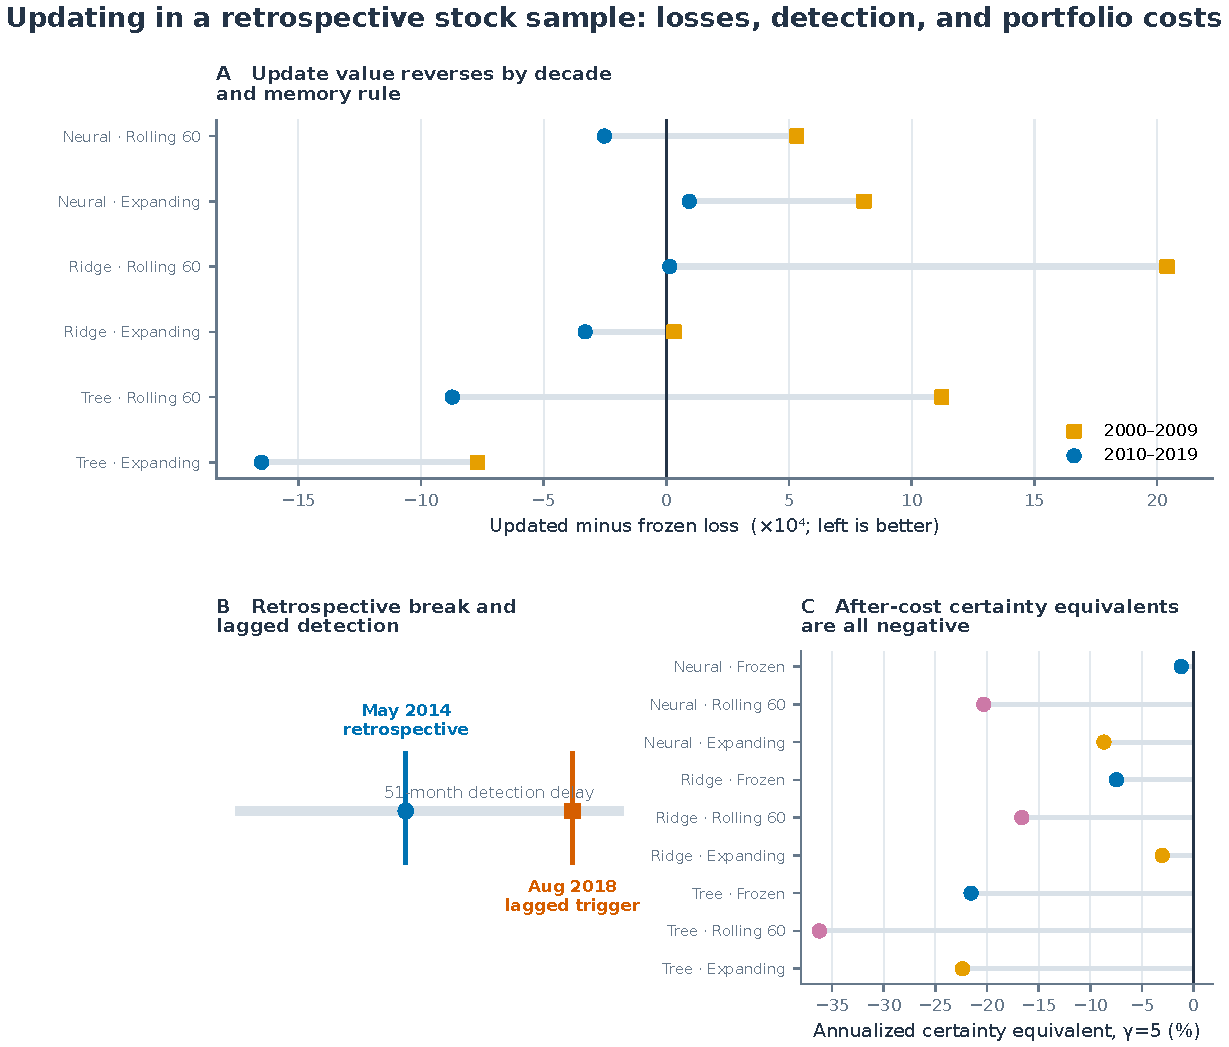
\includegraphics[width=0.99\textwidth]{../figures/figure_06_temporal_usability.pdf}
\caption{Temporal usability dashboard. Panel A reports updated-minus-frozen loss by learner, memory rule, and decade. Panel B contrasts the exploratory retrospective break with the frozen real-time CUSUM crossing. Panel C reports annualized certainty equivalents for the value-weighted 25-basis-point primary portfolios.}
\label{fig:temporal-dashboard}
\end{widefigure}

\subsubsection{Implication for temporal dimension claims}

Temporal instability does not imply that a researcher should continually change $K$ or retrain every parameter. A low-dimensional representation can remain geometrically compact while the risk prices attached to its directions, its asset exposures, or the usefulness of its forecast changes evolve. The current evidence locates a change in update alignment, but it does not yet separate exposure-span rotation from risk-price migration in the full 30-model family. That attribution is outside the evidence reported here.

For the evidence available here, the appropriate conclusion is narrower. Updating value varies over time and can be visible retrospectively. The tested lagged detector does not identify that change early enough to establish incremental value in this internal replay. Therefore a time-varying pattern cannot be used as evidence for a stable, real-time economic state variable unless the detection and implementation gates pass separately.


\section{Representation geometry and functional probe}
\setcounter{equation}{0}
The sample fixes 384 securities per development target month and uses the same rows in all 30 Core-86 models. There are 32,400 model--month--layer--normalization cells: 30 models, 120 months, three hidden layers, and three normalizations. Each spectral group has 3,600 observations. Adjacent-month drift has 3,570 observations per layer/normalization group, since there are 119 transitions. Neighbor diagnostics use January of each development year only, hence 300 observations per raw-centered or z-scored group; they are omitted under row normalization.

Let positive covariance eigenvalues be $\ell_j$, with $p_j=\ell_j/\sum_j\ell_j$. Participation rank is $(\sum_j\ell_j)^2/\sum_j\ell_j^2$; entropy rank is $\exp(-\sum_jp_j\log p_j)$; PCA90 and PCA95 are the smallest ranks reaching the stated variance shares. Numerical collapse is flagged if total variance is at most $10^{-12}$ or participation rank at most 1.05. This test does not assess the class-conditional geometry called neural collapse in supervised classification.

TWO-NN is the reciprocal mean log ratio of second to first neighbor distance, excluding invalid distances. The Levina--Bickel implementation uses the median local bias-adjusted estimate $(k-2)/\sum_{j<k}\log(r_k/r_j)$ at $k=20$. These estimators depend on sampling and neighborhood scale.

The variable archived as \texttt{curvature\_proxy\_radians} is a tangent-angle diagnostic. At eight deterministic random anchors it compares PCA tangents from 16 and 48 neighbors. Local rank is the rounded TWO-NN estimate clipped to 1--12 and further limited by the available coordinates. It reports the median largest principal angle between the two neighborhood scales. It is not a Weingarten-map curvature estimator and has no curvature units. Rank-five temporal Grassmann drift is the Euclidean norm of the five principal angles. Linear CKA is $\|X'Y\|_F^2/(\|X'X\|_F\|Y'Y\|_F)$ for centered activations.

The functional probe uses one median final-layer raw participation rank per model. The baseline is nominal-factor-count fixed effects; the augmented regression adds geometry. Each fold holds out one common seed across all six factor counts, leaving 24 training and six held-out models. The primary outcome is the normalized HJ span loss recorded in the frozen model report. This report-level endpoint refits span loadings for that evaluation report; it is distinct from the validation-fixed self-pricing distance in Figures 2--3. The probe predicts cross-model performance summaries, not next-month stock returns.

The permutation diagnostic shuffles geometry within factor count (5,000 draws; seed 7292026). The primary threshold requires at least 5\% leave-one-seed-out RMSE improvement and two-sided permutation $p\le0.05$. Observed improvement is 3.915\% and $p=0.149$. The secondary Sharpe probe has 1.211\% improvement and $p=0.041$, and cannot substitute for the primary endpoint. These 30 models share the economic period; five folds are algorithmic repetitions, not independent histories.

\subsection{Post-study random-network control}
Five fresh random hidden networks are evaluated on the same 120 sets of 384 securities as the 30 frozen trained networks. The inputs, 128--64--32 widths, SiLU activations, normalization rules, and seed identifiers match. For a given seed, hidden random weights are shared across all $K$ values and counted once in the random distribution. They are matched draws under the recorded control runtime, not asserted to be byte-identical to historical training initializations. The additional 5,400 random cells combine with 32,400 trained cells. Trained participation ranks and leading-eigenvalue shares match the earlier CPU replay to numerical precision.

The primary contrast is the raw-centered H3 mean participation rank divided by width, trained minus random. The means are 0.271584 and 0.324981, and the paired gap is $-0.053397$, with interval $[-0.077367,-0.033587]$. Each of 1,000 draws resamples common twelve-month circular blocks and paired seed clusters, retaining all six trained $K$ values inside their seed. The other layers, normalization rules, and leading-eigenvalue shares are descriptive. Inference is conditional on the archived sample and trained models, with five initialization clusters. The original functional endpoint, permutation test, and failure criterion are not changed by this control.

\section{Replication package and audit boundaries}
The public package is organized in article order: framework, data design, pricing dimension, temporal replay, and representation geometry. It includes all plotted aggregate data, numeric tables, synthetic selection outputs, methods code, configurations, dependency specifications, and a manifest of included file hashes. Restricted stock observations, historical benchmark security records, fitted weights, stock-level predictions, and individual-security intermediate panels are excluded. External freely downloadable inputs are referenced at their source with vintage hashes; accessibility alone is not a redistribution license.

The package distinguishes three operations. Exhibit replay reuses released aggregate inputs and regenerates figures, tables, and documents. Synthetic replay reruns the known-truth generator with its frozen seed and grid. Full empirical reconstruction requires licensed inputs matching the documented exports and historical vintages, together with the specified runtimes; exact numerical equality across hardware is not promised. Original execution receipts and protocol labels are retained alongside the chronology correction. No unexecuted attribution protocol is reported as evidence.

The manuscript audit additionally corrects three distinctions: 86 characteristics versus 172 network inputs; all-month spectral summaries versus ten-month neighbor diagnostics; and noisy-mean ``feasible'' simulation evaluation versus estimation of every population object. These corrections alter interpretation and documentation, not the archived experimental outcomes.
\end{document}
